\documentclass{btp}

\usepackage[T1]{fontenc}
\usepackage{caption}
\usepackage[superscript,biblabel]{cite}
\usepackage{minted}
\usepackage{url}
\usepackage{float}
\usepackage[xcolor,leftbars]{changebar}
\usepackage[nottoc,numbib]{tocbibind}
\usepackage{subcaption}

\usepackage{array}
\usepackage{multirow}
\usepackage{adjustbox}
\usepackage{makecell}

\newsavebox{\mintedbox}

\usepackage[linesnumbered, ruled]{algorithm2e}
\usepackage{algpseudocode}

\usepackage{tikz}
\usetikzlibrary{positioning, tikzmark, shapes, fit, calc}

\usepackage{graphicx}
\graphicspath{ {./images/} }

\usepackage{xcolor}
\definecolor{LightGray}{gray}{0.9}
\colorlet{LightRed}{red!20!white}
\colorlet{LightBlue}{blue!20!white}
\colorlet{LightGreen}{green!20!white}
\definecolor{ClassGreen}{HTML}{008000}
\definecolor{AnnoPurple}{HTML}{AA22FF}

\newcommand\mycommfont[1]{\footnotesize\ttfamily\textcolor{black!60!white}{#1}}
\SetCommentSty{mycommfont}

\usepackage[colorlinks = true,
            linkcolor = blue,
            urlcolor  = blue,
            citecolor = blue,
            anchorcolor = blue]{hyperref}


\usepackage{titling}

\makeatletter
\renewcommand\maketitle{%
%   \pagenumbering{roman}
%   \thispagestyle{empty}
  \newpage
  \null
%   \setcounter{page}{0}
%   \parskip=0pt
  \begin{center}%
  \let \footnote \thanks
  \vglue 0in % this makes top margin 2in
  \vskip -5ex%
    {\Large \bf \expandafter{\@title} \par}%
    \vskip 10ex%
    {\normalsize
           {\em A Project Report submitted by \par}
           \vskip 5ex%
           {\bf \large\MakeUppercase{\@author}\par\par}
           \vskip 5ex%
           {\normalsize \em in partial fulfillment of the requirements\par
             for the award of the degree of \par}
           \vskip 5ex%
              {\bf BACHELOR OF TECHNOLOGY}
    }
  \end{center}%

  \vspace*{0.75in}
  %\centerline{\psfig{figure=emblem.ps}}
%  \centerline{\includegraphics{iitm.eps}}
  \centerline{\includegraphics[scale=1.]{iitm}}
%   \vspace*{-0.15in}
  \begin{center}
    {\bf \large DEPARTMENT OF COMPUTER SCIENCE AND ENGINEERING\par}
    {\bf \large INDIAN INSTITUTE OF TECHNOLOGY MADRAS.}
    \vglue 0.50em
    {\bf \large \@date}\par
  \end{center}
%   \parskip 8pt
}
\makeatother

\setlength{\parindent}{0pt}

\title{\Huge Adding ThreadSanitizer support in LLVM backend for AMD GPUs}
\author{{\huge Dhruv Maroo} \\ {\Large Advised by Prof. Rupesh Nasre}}

\begin{document}

\maketitle
\newpage

\begin{abstract}
	\noindent With the rise of ROCm, AMD's open-source GPU programming stack, there has been a lot of focus on improving AMD's developer experience when programming on AMD GPUs. One of the main, and recommended, languages for such programming is AMD's HIP. It can be seen as a language similar to CUDA, but with support for multiple backends including AMD GPU.
	\\
	\newline
	LLVM has support for compiling HIP code to generate AMDGCN code, which can be run on AMD GPUs. Having LLVM support also means that the compilation leverages other LLVM features, like optimizations, MLIR generation, AddressSanitizer and so on. But, unfortunately, there is no ThreadSanitizer support for code being compiled for AMD GPUs. Given that majority of the code being compiled for AMD GPU is parallel code, it makes addition of ThreadSanitizer a game-changing improvement in terms of developer experience and reliability.
	\\
	\newline
	In this report, I go over my attempt to implement a subset of ThreadSanitizer for the AMD GPU backend. I go over the prior research regarding this and their conclusions. I also write about how ThreadSanitizer fits in the LLVM toolchain. I go over the problems that I faced during the implementation of ThreadSanitizer. I also go over the algorithm used under the hood and their proof-of-concept GPU implementations. Following this, I benchmark these proof-of-concept implementations in terms of the space and time overhead. Finally, I end with possible future work and improvements upon the initial design and implementation.
\end{abstract}

\tableofcontents

\newpage

\section{Introduction}

Parallel programming is growing in popularity day by day, more so with the advent of multi-code CPUs and GPUs. This is because of the magnitude of speedup obtained by parallelizing computationally heavy code. Moreover, use of GPUs for computation purposes has also increased in the scientific computing, high-performance computing and game development scene.
\\
\newline
However, writing parallel code is not easy. There are countless pitfalls when it comes to writing bug-free parallel code, ranging from data races, to synchronization issues. All of these issues are sometimes non-trivial to find and debug. Due to this, there has been extensive research and tooling developed to help programmers avoid such pitfalls. More specifically, much of the tooling is built for detecting data races through either static or dynamic analysis techniques.
\\
\newline
ThreadSanitizer \cite{tsan-llvm} is one such tool. It is integrated with the LLVM compiler toolchain, and hence is very easy to use or deploy right out of the box. Moreover, it is a dynamic race detection tool, and hence is very effective and quick at pinpointing races during the execution. It also supports a lot of the modern architectures.
\\
\newline
But the common thing among all such tools is that none of them support any of the GPU architectures. GPUs are built for parallel code execution and thus it would be expected that there would be rich tooling for detecting GPU races. But that is not the case, since most of the race detection tools, including ThreadSanitizer support only CPU architectures.
\\
\newline
This has led to scattered support of race detection tools in the GPU programming space, many of which are either proprietary or have any other sort of vendor lock-in. There is no ThreadSanitizer equivalent for GPUs. This was main reason behind pursuing this idea further.

\section{Motivation}

\subsection{Why AMD GPUs?}

One of the biggest GPU design/manufacturing company is \textsc{Nvidia}. \textsc{Nvidia} has a very rich and mature developer ecosystem, consisting of variety of tools, utilities and abundant documentation leading to a great developer experience. This has also led to better code, in terms of safety, quality, maintainability, efficiency and so on. Similarly, AMD is a behemoth as well, when it comes to building processors, and GPUs as well.
\\
\newline
Moreover, due to ROCm \cite{rocm}, AMD's open-source GPU programming stack, there has been an increased interest in programming on AMD GPUs. Along with this, their HIP \cite{hip} SDK also makes it really easy to write architecture agnostic parallel code, since it supports multiple backends, including \textsc{Nvidia}'s CUDA \cite{cuda} backend.

\subsection{Why ThreadSanitizer?}

If we look at \textsc{Nvidia}'s CUDA developer tools, we can see that they provide a rich ecosystem of developer tools. For profilers, they provide \texttt{nvprof} and the NSight's visual profiler\cite{nvprof}. For debugging tools, they provide CUDA-GDB \cite{cudagdb} debugger for CUDA code, and the \texttt{compute-sanitizer} \cite{compsan} for sanitizing CUDA code. \texttt{compute-sanitizer} supports multiple checkers like a memory/address checker, race checker, uninitialized value checker and synchronization checker.
\\
\newline
On the other hand, for AMD GPUs, there is \texttt{rocprofiler} \cite{rocprofiler} for profiling, and ROCgdb \cite{rocgdb} for debugging. AddressSanitizer support \cite{asan-amdgpu} for AMD GPU was also recently upstreamed to LLVM \cite{asan-patch-amd}. However, there is no equivalent of ThreadSanitizer in case of AMD GPUs. This prompted to work on implementing ThreadSanitizer support for AMD GPUs as my B. Tech project.

\begin{minted}
[
frame=lines,
framesep=2mm,
numbersep=5pt,
baselinestretch=1.1,
bgcolor=LightGray,
fontsize=\footnotesize,
]
{text}
$ compute-sanitizer --help
NVIDIA (R) Compute Sanitizer
Copyright (c) 2020-2024 NVIDIA Corporation
Version 2024.1.1.0 (build 34043715) (public-release)
Usage: compute-sanitizer [options] [your-program] [your-program-options]

General options:
  -h [ --help ]                         Produce this help message.

...

  --tool arg (=memcheck)                Set the tool to use.
                                        memcheck  : Memory access checking
                                        racecheck : Shared memory hazard checking
                                        synccheck : Synchronization checking
                                        initcheck : Global memory initialization checking

...

Please see the compute-sanitizer manual for more information.

$ nvcc racefree.cu -o racefree
$ compute-sanitizer --tool racecheck -- ./racefree
========= COMPUTE-SANITIZER
========= RACECHECK SUMMARY: 0 hazards displayed (0 errors, 0 warnings)
\end{minted}

\section{Prior work}

\subsection{CUDA \texttt{compute-sanitizer}}

The \texttt{compute-sanitizer} is a versatile tool as explained above. But we are only focused on the \textit{racecheck} functionality of the tool. Racecheck works by instrumenting the binary being run, therefore adding hooks for any accesses and using dynamic race detection algorithms on the resulting trace to find any data races. This allows us to run existing binaries through racecheck without compilation.
\\
\newline
This sort of instrumentation is done through the \texttt{LD\_PRELOAD} environment variable. This allows programmers to override the dynamic libraries being loaded. We can use this to override the \texttt{\_\_cudaRegisterFatBinary()} function from the CUDA runtime. This function is responsible for loading the embedded CUDA fat binary onto the GPU. This function call can be intercepted and the binary which is being loaded can be modified on-the-fly to insert instrumentation. In fact, this is how NVBit \cite{nvbit} (NVidia Binary Instrumentation Tool), an open source tool, also does it.
\\
\newline
The problem with this approach is that it is completely detached with the compilation process, and is somewhat hacky. Ideally, binary instrumentation on the CPU is usually done at the compilation stage, which is how it should also be done for the GPU code. Moreover, \texttt{compute-sanitizer} misses many benign races including global memory and only effectively works for \texttt{\_\_shared\_\_} memory.

\subsection{\textsc{ScoRD}: A Scoped Race Detector for GPUs}

\textsc{ScoRD} \cite{scord} is a race detector that enables hardware support for efficiently detecting global memory races in a GPU program, including those that arise due to insufficient scopes of synchronization operations. The authors claim that ScoRD can detect a variety of races and has an average performance overhead of 35\%.
\\
\newline
The main idea is to modify the hardware and the runtime to store extra information during kernel execution which can be used to detect races. This extra information includes locks' statuses, access information, synchronization information and so on. The main problem with this approach is that it requires hardware extensions and modifications at the runtime level, which may not be feasible and maintanable in the long run.

\subsection{Predictive Data Race Detection for GPUs}

This paper talks about the tool \texttt{PreDataR} \cite{iitk}, which is used detect data races in the program dynamically. They instrument the binary with this tool and keep track of all the GWCP relations (which stands for GPU weak-causally-precedes). These relations are constructed during the run through the instrumented hooks, and later these relations are used to perform predictive data race detection.
\\
\newline
The authors have developed the tools for \textsc{Nvidia} GPUs however. They use NVBit for \textsc{Nvidia} binary instrumentation. They also employ compressed vector clocks to keep track of the GWCP ordering.

\subsection{\textsc{Barracuda}: Binary-level Analysis of Runtime RAces in CUDA programs}

\textsc{Barracuda} \cite{barracuda} is a tool developed to find data races in CUDA programs. This done by performing binary instrumention on the CUDA code at the PTX level. Therefore, since the instrumentation is at the PTX level, it can also be applied to existing binaries without recompilation.
\\
\newline
The algorithm is somewhat similar to ThreadSanitizer's \nameref{sec:algo}. The algorithm also uses hooks to keep track of accesses, uses happens-before relations, but it uses vector clocks for each of the threads. They claim that the overhead of \textsc{Barracuda} is comparable to \texttt{compute-sanitizer} racecheck's overhead.

\subsection{\textsc{iGuard}: In-GPU Advanced Race Detection}

\textsc{iGuard} \cite{iguard} is another runtime race detection tool for CUDA code being run on \textsc{Nvidia} GPUs. It also uses NVBit to instrument binaries and add hooks for memory accesses and synchronization operations.
\\
\newline
It also uses happens-before relations and a lockset algorithm to keep track of locks. Using information from both of these sources, it is able to detect races effectively. Moreover, it claims to be faster than other alternatives like \textsc{Barracuda} since the entire race detection is done in parallel over the GPU rather than in a sequential manner.

\section{Goal}

The main goal of the project was to explore the feasibility and have a prototype dynamic race detector working for AMD GPUs. Ideally, we would want to be able to detect and report races just like \textsc{Nvidia} compute-sanitizer's racecheck. Along with this, we should also be able to run the race detector on benchmarks and get a rough measure of the overheads introduced.

\section{Understanding the ROCm ecosystem}

\subsection{What is ROCm?}

ROCm \cite{rocm} is AMD's open-source software stack for GPU programming. It is a collection of a kernel language (HIP), programming libraries and toolchains and runtime APIs for GPU programming. For the most part of the project, we need not deal with the ROCm programming libraries and runtime APIs. HIP, however, is an important component of the ROCm stack.

\subsection{What is HIP?}

HIP stands for \textit{Heterogeneous-Compute Interface for Portability}. As the name suggests, it is a set of kernel language, APIs and programming libraries to be used for writing computational code, with portability as one of the goals. Quoting HIP's source repository \cite{hip-github}, these are the key features provided by HIP.

\begin{quote}
	\begin{changebar}\cbcolor{gray}\color{black}
		Key features include:

		\begin{itemize}
			\item HIP is very thin and has little or no performance impact over coding directly in CUDA mode.
			\item HIP allows coding in a single-source C++ programming language including features such as templates, C++11 lambdas, classes, namespaces, and more.
			\item HIP allows developers to use the "best" development environment and tools on each target platform.
			\item The HIPIFY tools automatically convert source from CUDA to HIP.
			\item Developers can specialize for the platform (CUDA or AMD) to tune for performance or handle tricky cases.
		\end{itemize}
	\end{changebar}
\end{quote}

The main idea for HIP is to be a flexible and portable programming environment providing great support for migration of CUDA codebases. In fact, as mentioned in the features, there is a tool to convert CUDA code to HIP code, HIPIFY \cite{hipify}.

\subsection{HIPCC}
\label{sec:hipcc}

HIPCC is a compiler driver utility for HIP code. It can be used to compile HIP code for both the targets, AMD GPU and \textsc{Nvidia} GPU. You can specify the desired target at compile time using the \texttt{HIP\_PLATFORM} environment variable.
\\
\newline
HIPCC is not a full-fledged compiler, rather, it is just a wrapper which calls either \texttt{nvcc} (\textsc{Nvidia}'s compiler for CUDA code) or calls \texttt{clang}. Due to its simplicity, HIPCC has been implemented as both, a Perl script and a C++ binary. HIPCC is mainly responsible to passing the correct arguments to \texttt{clang}. These arguments set many flags which would otherwise be tedious to set manually. A simple compilation command as follows,

\begin{minted}
	[
	frame=lines,
	framesep=2mm,
	numbersep=5pt,
	baselinestretch=1.0,
	bgcolor=LightGray,
	fontsize=\footnotesize,
	]
	{text}
$ /opt/rocm/bin/hipcc demo.cpp -o demo
\end{minted}

gets expanded into a huge complex command with multiple arguments and flags as follows.

\begin{minted}
[
frame=lines,
framesep=2mm,
numbersep=5pt,
baselinestretch=1.0,
bgcolor=LightGray,
fontsize=\scriptsize,
breaklines,
escapeinside=||
]
{text}
"/opt/rocm/lib/llvm/bin/clang-17" -cc1 -triple amdgcn-amd-amdhsa -aux-triple x86_64-pc-linux-gnu -emit-obj -disable-free -clear-ast-before-backend -main-file-name demo.cpp -mrelocation-model pic -pic-level 2 -fhalf-no-semantic-interposition -mframe-pointer=none -fno-rounding-math -mconstructor-aliases -aux-target-cpu x86-64 -fcuda-is-device -mllvm -amdgpu-internalize-symbols -fcuda-allow-variadic-functions -fvisibility=hidden -fapply-global-visibility-to-externs -mlink-builtin-bitcode /opt/rocm/amdgcn/bitcode/hip.bc -mlink-builtin-bitcode /opt/rocm/amdgcn/bitcode/ocml.bc -mlink-builtin-bitcode /opt/rocm/amdgcn/bitcode/ockl.bc -mlink-builtin-bitcode /opt/rocm/amdgcn/bitcode/oclc_daz_opt_off.bc -mlink-builtin-bitcode /opt/rocm/amdgcn/bitcode/oclc_unsafe_math_off.bc -mlink-builtin-bitcode /opt/rocm/amdgcn/bitcode/oclc_finite_only_off.bc -mlink-builtin-bitcode /opt/rocm/amdgcn/bitcode/oclc_correctly_rounded_sqrt_on.bc -mlink-builtin-bitcode /opt/rocm/amdgcn/bitcode/oclc_wavefrontsize64_on.bc -mlink-builtin-bitcode /opt/rocm/amdgcn/bitcode/oclc_isa_version_90c.bc -mlink-builtin-bitcode /opt/rocm/amdgcn/bitcode/oclc_abi_version_500.bc -target-cpu gfx90c -debugger-tuning=gdb -resource-dir /opt/rocm/lib/llvm/lib/clang/17.0.0 -internal-isystem /opt/rocm/lib/llvm/lib/clang/17.0.0/include/cuda_wrappers -idirafter /opt/rocm/include -include __clang_hip_runtime_wrapper.h -c-isystem /opt/rocm/llvm/include/gpu-none-llvm -isystem /opt/rocm/include -internal-isystem /usr/lib64/gcc/x86_64-pc-linux-gnu/13.2.1/../../../../include/c++/13.2.1 -internal-isystem /usr/lib64/gcc/x86_64-pc-linux-gnu/13.2.1/../../../../include/c++/13.2.1/x86_64-pc-linux-gnu -internal-isystem /usr/lib64/gcc/x86_64-pc-linux-gnu/13.2.1/../../../../include/c++/13.2.1/backward -internal-isystem /usr/lib64/gcc/x86_64-pc-linux-gnu/13.2.1/../../../../include/c++/13.2.1 -internal-isystem /usr/lib64/gcc/x86_64-pc-linux-gnu/13.2.1/../../../../include/c++/13.2.1/x86_64-pc-linux-gnu -internal-isystem /usr/lib64/gcc/x86_64-pc-linux-gnu/13.2.1/../../../../include/c++/13.2.1/backward
|$\scriptstyle{\hookrightarrow}$\:\:| -internal-isystem /opt/rocm/lib/llvm/lib/clang/17.0.0/include -internal-isystem /usr/local/include -internal-isystem /usr/lib64/gcc/x86_64-pc-linux-gnu/13.2.1/../../../../x86_64-pc-linux-gnu/include -internal-externc-isystem /include -internal-externc-isystem /usr/include -internal-isystem /opt/rocm/lib/llvm/lib/clang/17.0.0/include -internal-isystem /usr/local/include -internal-isystem /usr/lib64/gcc/x86_64-pc-linux-gnu/13.2.1/../../../../x86_64-pc-linux-gnu/include -internal-externc-isystem /include -internal-externc-isystem /usr/include -O3 -fdeprecated-macro -fno-autolink -ferror-limit 19 -fhip-new-launch-api -fgnuc-version=4.2.1 -fcxx-exceptions -fexceptions -fcolor-diagnostics -vectorize-loops -vectorize-slp -mllvm -amdgpu-early-inline-all=true -mllvm -amdgpu-function-calls=false -cuid=ad64b8986ed345d9 -fcuda-allow-variadic-functions -faddrsig -D__GCC_HAVE_DWARF2_CFI_ASM=1 -o /tmp/demo-gfx90c-68a3a2.o -x hip demo.cpp
\end{minted}

This expanded command can be obtained by passing the \texttt{-v} flag to \texttt{hipcc}. The flag stands for verbosity and will print all the commands being invoked and the environment variables being used. Now, we can find some interesting flags in the above command.

\begin{itemize}
	\item \texttt{-triple amdgcn-amd-amdhsa}: This is specifying the LLVM target triple \cite{triple}. Target triples consist information about the architecture, vendor, OS, platform, ABI and so on.
	\item \texttt{-aux-triple x86\_64-pc-linux-gnu}: This is the auxiliary target triple. In this case, it refers to the host system's triple. Since I'm using a 64-bit Linux machine, my target triple is \texttt{x86\_64-pc-linux-gnu}.
	\item \texttt{-aux-target-cpu x86-64}: This is a CUDA and HIP specific flag passed in to keep track of the host CPU.
	\item \texttt{-target-cpu gfx90c}: This specifies the target AMD GPU for which the code is being compiled. The exhaustive list and more documentation can be found in the LLVM docs \cite{llvm-amd-docs}.
	\item \texttt{-mlink-builtin-bitcode}: This flag is repeated a bunch of times, and is followed by AMD GPU bitcode files. These files contain the implementations for the HIP builtins.
	\item \texttt{-internal-isystem}: This flag is used to add directories to internal system include search paths.
\end{itemize}

In the case that you don't have ROCm toolchain present, HIPCC detects whether you have \texttt{nvcc} installed on your machine. If you do, then it uses \texttt{nvcc} to generate code for \textsc{Nvidia} GPU. The expanded \texttt{nvcc} is much shorter compared to its \texttt{clang} counterpart.

\begin{figure}[H]
	\centering
	\begin{tikzpicture}
		\node (rocmRec)[rectangle, draw, minimum height = 7cm, minimum width = 15cm] { };
		\node (rocmLibs)[rectangle, draw, align=center, minimum height = 5cm, minimum width = 4cm, below right=-2cm and 0.75cm of rocmRec.west] { rocFFT, rocBLAS, \\ rocRAND, rocPRIM, \\ rocSOLVER, rocThrust, \\ rocHPL };
		\node (hip)[rectangle, draw, align=center, minimum height = 5cm, minimum width = 4cm, below right=-2cm and 5.5cm of rocmRec.west] { HIPCC, HIPIFY, \\ hip-python, hipBLAS, \\ hipFFT, hipSolver, \\ hipTensor, hipRAND, \\ hipSPARSE };
		\node (rocmAPI)[rectangle, draw, align=center, minimum height = 5cm, minimum width = 4cm, below right=-2cm and 10.25cm of rocmRec.west] {
			\begin{minipage}{3cm}
				\vspace*{0.5cm}
				AMD CLR -\\ Compute Language\\ Runtimes
				\begin{itemize}
					\item \texttt{hipamd}
					\item \texttt{opencl}
					\item \texttt{rocclr}
				\end{itemize}
			\end{minipage}
		};
		\node (hipRect)[rectangle, draw, fill=LightRed, minimum height = 1cm, minimum width = 3cm, below right=1.75cm and 6cm of rocmRec.west] { HIPCC };
		\node (llvmRect)[rectangle, draw, text width=2cm, fill=LightBlue, minimum height = 1cm, minimum width = 3cm, below left=1cm and 1cm of hipRect] { \texttt{llvm} };
		\node (nvccRect)[rectangle, draw, text width=2cm, fill=LightGreen, minimum height = 1cm, minimum width = 3cm, below right=1cm and 1cm of hipRect] { \texttt{nvcc} };


		\node (rocmText) [below=0.25cm of rocmRec.north] { \large \textbf{ROCm ecosystem} };
		\node (rocmImage) [below left=0.15cm and 0.2cm of rocmRec.north east] { \includegraphics[width=.05\textwidth]{rocm.png} };
		\node (hipTitle)[below=0.15cm of hip.north] { \textbf{HIP language} };
		\node (rocmLibsTitle)[below=0.15cm of rocmLibs.north] { \textbf{ROCm libraries} };
		\node (rocmAPITitle)[below=0.15cm of rocmAPI.north] { \textbf{ROCm runtime} };
		\node (platformEnv) [below right=0.25cm and 0cm of hipRect.south] { \texttt{HIP\_PLATFORM} };
		\node (llvmImage) [below left=0.2cm and 0.3cm of llvmRect.north east] { \includegraphics[width=0.7cm]{LLVM_logo.png} };
		\node (llvmImage) [below left=0cm and 0.3cm of nvccRect.north east] { \includegraphics[width=0.7cm]{nvidia-logo.png} };

		\draw[-latex] (hipRect) |- (llvmRect) node[pos=0.75, below](platformLLVM){\texttt{amd}};
		\draw[-latex] (hipRect) |- (nvccRect) node[pos=0.75, below](platformNVCC){\texttt{nvidia}};
	\end{tikzpicture}

	\caption{ROCm ecosystem with all the major components.}
\end{figure}

\subsection{Example}

Due to the need for compatibility with \texttt{nvcc}, HIP code is very similar to CUDA code. A lot of the syntax is similar and so are language specific identifiers. This allows for easy interoperability with CUDA. In fact, HIPIFY is just a Perl script (also available as a Python script) which performs text operations on the CUDA code to convert it to HIP.

\subsubsection{HIP kernel}

An example kernel would be as follows.

\begin{minted}
[
frame=lines,
framesep=2mm,
numbersep=5pt,
baselinestretch=1.0,
bgcolor=LightGray,
fontsize=\footnotesize,
linenos
]
{cuda}
__global__ void compute(int *array, int *count, int value) {
	int index = threadIdx.x + blockIdx.x * blockDim.x;

	int updateValue;
	if (index % 2 == 1) {
		updateValue = value;
	} else {
		updateValue = value - 3;
	}

	array[index] += updateValue;
	atomicAdd(count, 1);
}
\end{minted}

In the above kernel, you can identify the uses of \texttt{threadIdx.x}, \texttt{blockIdx.x} and \texttt{blockDim.x} if you're familiar with CUDA code. In HIP code as well, these variables denote the same thing. Moreover, even the builtins, like \texttt{atomicAdd}, possess the same name as their CUDA counterpart.

\subsubsection{HIP API}

The HIP APIs which are used to copy data, call kernels and so on, are also similarly named to their CUDA equivalent. The only difference is that the functions in the API start with the \texttt{hip} prefix rather than the \texttt{cuda} prefix of their CUDA counterparts. The same is also true for HIP enums and types. We can observe it in the following example code, which calls the compute kernel we defined above.

\begin{minted}
[
frame=lines,
framesep=2mm,
numbersep=5pt,
baselinestretch=1.0,
bgcolor=LightGray,
fontsize=\footnotesize,
linenos
]
{c++}
#include <hip/hip_runtime.h>

__global__ void compute(int *array, int *count, int value) { ... }

int main(int argc, char *argv[]) {
    int *d_array;
    hipMalloc(&d_array, SIZE * sizeof(*d_array));

    int h_array[SIZE] = { ... };
    hipMemcpy(d_array, h_array, SIZE * sizeof(*h_array), hipMemcpyHostToDevice);

    int *d_count;
    hipMalloc(&d_count, sizeof(*d_count));
    hipMemset(d_count, 0, sizeof(*d_count));

    compute<<<1, SIZE>>>(d_array, d_count, 7);
    hipDeviceSynchronize();

    int h_result[SIZE];
    hipMemcpy(h_result, d_array, SIZE * sizeof(*d_array), hipMemcpyDeviceToHost);

	...
}
\end{minted}

\section{LLVM}

LLVM is a compiler framework/infrastructure built with extensibility in mind. LLVM modularized multiple aspects and stages of compilation. LLVM can be mainly divided into 2 parts, the frontend and the backend.

\subsection{Frontend}

The main responsibility of the frontend is to handle all the steps before the machine code generation. However, practically speaking, not everything before machine code generation is completely considered part of the frontend. The main stages of the frontend can be classified as follows.

\begin{itemize}
	\item \textbf{Parse command-line arguments:} All the command-line flags/arguments are supposed to be parsed by the frontend. We need to modify a little bit of the frontend so that we can add a new flag for GPU thread sanitization (\texttt{-fgpu-sanitize=thread}). We cannot reuse the existing thread sanitization flag (\texttt{-fsanitize=thread}) because it is meant to instrument CPU code. We may sometimes want to just instrument the GPU code without instrumenting the GPU code, in which case we should use the GPU specific flag.
	\item \textbf{Tokenize and parse the code:} It is also the frontend's responsibility to tokenize and parse the code. Hence, any syntax error would, thus, be detected by the frontend. Moreover, any parsing error, which could include unused variables or type mismatch, would also be detected by the frontend.
	\item \textbf{MLIR generation:} Post parsing, the frontend should generate the MLIR \cite{mlir} (\textit{Multi-level Intermediate Representation}) code from the input source. This MLIR code will then be passed on to the backend. MLIR code can be seen as the frontend and the backend's communication language.
\end{itemize}

\subsection{Backend}

The LLVM backend is primarily responsible for transforming the MLIR code, performing optimizations and finally generating machine code for the target architecture. All the instrumentation for ThreadSanitizer (or for that matter, any other sanitizer) is done in the backend. The main stages of the backend can be classified as follows.

\begin{itemize}
	\item \textbf{MLIR transformations:} MLIR transformations can be seen as operations which take in MLIR code and output different MLIR code (or loosely speaking, some other level IR code). These usually consist of all sorts of optimization and instrumentation passes. And this is where thread sanitizer also comes in play.
	\item \textbf{Machine-code generation:} This is the part where the MLIR is finally lowered down to machine-code. This process also consists of multiple passes, like instruction selection, register allocation, architecture-specific optimization passes and so on. Thanks to LLVM's modular architecture, we do not need to touch the machine-code generation pass for adding thread sanitizer support.
\end{itemize}

\subsection{Linking}

Once the backend generates the machine code, the LLVM linker (\texttt{lld}) links the generated code with the relevant libraries and the runtime. For C/C++ code, these libraries usually are \texttt{libc} and \texttt{libc++}. These libraries are mostly platform dependent. Other languages (like Rust and Go) have their own set of runtime libraries which they link to.
\\
\newline
In case of HIP code, as we observed in the expanded LLVM command generated by \texttt{hipcc}, we link with host HIP libraries (which contain implementations for the HIP APIs) and with device libraries as well. These device libraries also contain the ASAN (address sanitizer) runtime libraries (you can find them at \texttt{amd/device-libs/asanrtl/} in the AMD's LLVM fork \cite{amd-llvm-fork}). Similarly, the thread sanitizer also has a runtime library which contains implementations for all the hooks. which get inserted by the backend. During the linking stage this runtime library gets linked with the instrumented binary.

\begin{figure}[H]
	\centering
	\makebox[\textwidth][c]{
	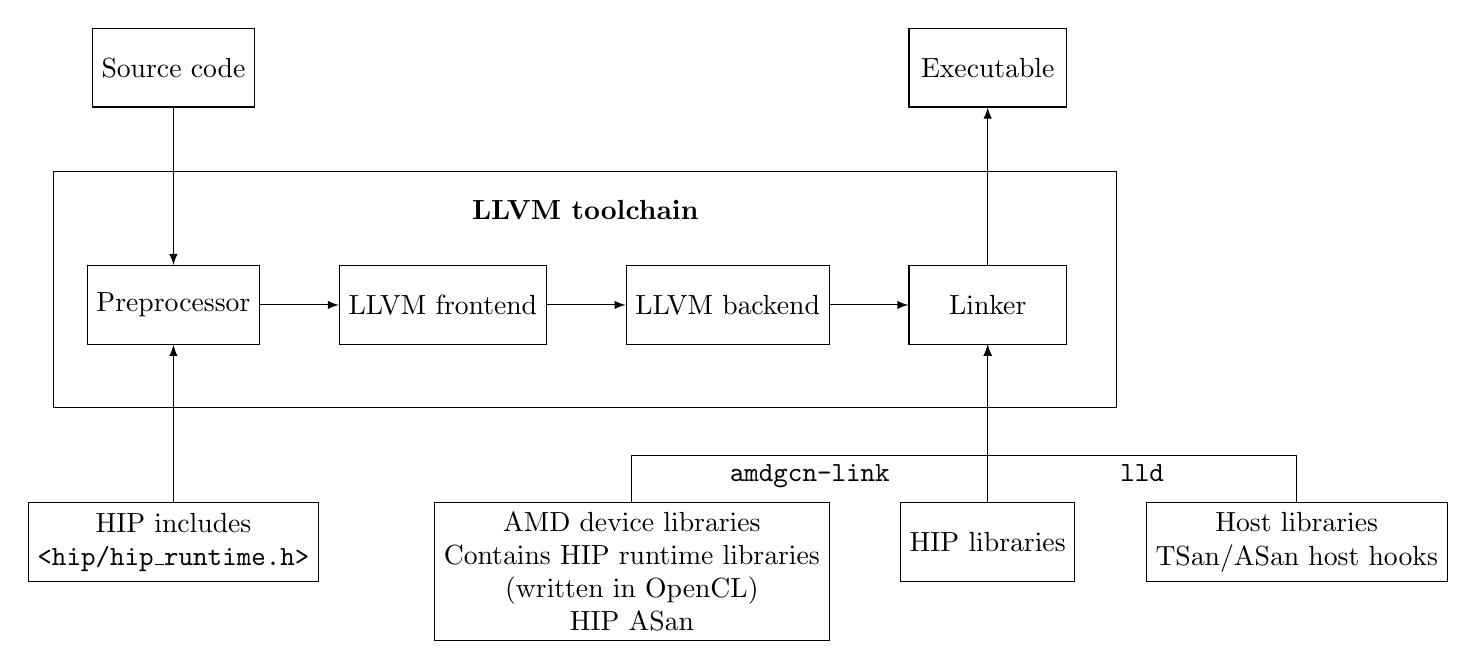
\begin{tikzpicture}
		\node (sourceCode)[rectangle, draw, minimum height = 1cm, minimum width = 2cm] { Source code };
		\node (preprocessor)[rectangle, draw, minimum height = 1cm, minimum width = 2cm, below=2cm of sourceCode] { Preprocessor };
		\node (frontend)[rectangle, draw, minimum height = 1cm, minimum width = 2cm, right=of preprocessor] { LLVM frontend };
		\node (backend)[rectangle, draw, minimum height = 1cm, minimum width = 2cm, right=of frontend] { LLVM backend };
		\node (linker)[rectangle, draw, minimum height = 1cm, minimum width = 2cm, right=of backend] { Linker };
		\node (executable)[rectangle, draw, minimum height = 1cm, minimum width = 2cm, above=2cm of linker] { Executable };
		\node (hipIncludes)[rectangle, draw, align=center, minimum height = 1cm, minimum width = 2cm, below=2cm of preprocessor] { HIP includes \\ \texttt{<hip/hip\_runtime.h>}};
		\node (amdDevLibs)[rectangle, draw, align=center, minimum height = 1cm, minimum width = 2cm, below left=2cm and 1cm of linker] { AMD device libraries \\ Contains HIP runtime libraries \\ (written in OpenCL) \\ HIP ASan};
		\node (hipLibs)[rectangle, draw, align=center, minimum height = 1cm, minimum width = 2cm, below=2cm of linker] { HIP libraries};
		\node (hostLibs)[rectangle, draw, align=center, minimum height = 1cm, minimum width = 2cm, below right=2cm and 1cm of linker] { Host libraries \\ TSan/ASan host hooks};
		\node (llvmToolchain)[rectangle, draw, minimum height = 3cm, minimum width = 13.5cm, yshift=0.2cm] at ($(frontend)!0.5!(backend)$) {};
		\node (llvmText)[below=0.25cm of llvmToolchain.north] {\textbf{LLVM toolchain}};
		
		\draw[-latex] (sourceCode) -- (preprocessor) {};
		\draw[-latex] (hipIncludes) -- (preprocessor) {};
		\draw[-latex] (preprocessor) -- (frontend) {};
		\draw[-latex] (frontend) -- (backend) {};
		\draw[-latex] (backend) -- (linker) {};
		\draw[-latex] (linker) -- (executable) {};
		\draw[-latex] (hipLibs) -- (linker) {};
		\draw[-latex] (amdDevLibs.north) -- +(0, 0.6) -| (linker) node[pos=0.25, below](amdDevLink){\texttt{amdgcn-link}};
		\draw[-latex] (hostLibs.north) -- +(0, 0.6) -| (linker) node[pos=0.25, below](hostLink){\texttt{lld}};
	\end{tikzpicture}
	}

	\caption{Compilation lifecycle when using LLVM.}
\end{figure}

\subsection{MLIR}

MLIR is LLVM's intermediate language. All the different intermediate languages in LLVM are implemented as dialects of MLIR. This MLIR code is architecture and programming language agnostic. For example, the LLVM MLIR code for both host and device code is the same. You can confirm this by looking through the table on the next page.
\\
\newline
Most of the optimization and transformation passes are performed over MLIR code. The ThreadSanitizer also inserts all the instrumentation hooks at the MLIR level. As an example, we can see how the following HIP kernel gets compiled to MLIR and the MLIR gets instrumented by ThreadSanitizer.

\begin{table}[H]
	\caption {Effect of ThreadSanitizer instruementation on MLIR.}
	\begin{adjustbox}{center}
		{\renewcommand{\arraystretch}{1.2}
			\begin{tabular}{|>{\hspace{0.3cm}}c|>{\hspace{0.3cm}}c|>{\hspace{0.3cm}}c|}
				\hline
				Source code                                                                                                     & MLIR code & Instrumented MLIR code \\
				\hline
				\begin{minipage}[t]{0.25\textwidth}
					\begin{minted}
			[
			frame=lines,
			framesep=2mm,
			numbersep=5pt,
			baselinestretch=1.0,
			bgcolor=LightGray,
			fontsize=\tiny,
			breaklines,
			linenos
			]
			{cuda}
__global__ void simple(int *a) {
	*a = 42;
}
			\end{minted}
				\end{minipage}                                                                             &
				\begin{minipage}[t]{0.375\textwidth}
					\begin{minted}
			[
				frame=lines,
				framesep=2mm,
				numbersep=5pt,
				baselinestretch=1.0,
				bgcolor=LightGray,
				fontsize=\tiny,
				breaklines,
				linenos
			]
			{text}
define protected amdgpu_kernel void @_Z10helloworldPi(ptr addrspace(1) noundef %0) #4 {
  %2 = alloca ptr, align 8, addrspace(5)
  %3 = alloca ptr, align 8, addrspace(5)
  %4 = addrspacecast ptr addrspace(5) %2 to ptr
  %5 = addrspacecast ptr addrspace(5) %3 to ptr
  %6 = addrspacecast ptr addrspace(1) %0 to ptr
  store ptr %6, ptr %4, align 8
  %7 = load ptr, ptr %4, align 8
  store ptr %7, ptr %5, align 8
  %8 = load ptr, ptr %5, align 8
  store i32 42, ptr %8, align 4
  ret void
}
			\end{minted}
				\end{minipage} &
				\begin{minipage}[t]{0.375\textwidth}
					\begin{minted}
			[
				frame=lines,
				framesep=2mm,
				numbersep=5pt,
				baselinestretch=1.0,
				bgcolor=LightGray,
				fontsize=\tiny,
				breaklines,
				linenos,
				highlightlines={3, 13, 15},
				highlightcolor=LightBlue
			]
			{text}
define protected amdgpu_kernel void @_Z10helloworldPi(ptr addrspace(1) noundef %0) #4 {
  %2 = call ptr @llvm.returnaddress(i32 0)
  call void @__tsan_func_entry(ptr %2)
  %3 = alloca ptr, align 8, addrspace(5)
  %4 = alloca ptr, align 8, addrspace(5)
  %5 = addrspacecast ptr addrspace(5) %3 to ptr
  %6 = addrspacecast ptr addrspace(5) %4 to ptr
  %7 = addrspacecast ptr addrspace(1) %0 to ptr
  store ptr %7, ptr %5, align 8
  %8 = load ptr, ptr %5, align 8
  store ptr %8, ptr %6, align 8
  %9 = load ptr, ptr %6, align 8
  call void @__tsan_write4(ptr %9)
  store i32 42, ptr %9, align 4
  call void @__tsan_func_exit()
  ret void
}
			\end{minted}
				\end{minipage}                                      \\
				\hline
			\end{tabular}}
	\end{adjustbox}
\end{table}

\begin{table}[H]
	\caption {Comparison of MLIR generated from HIP code and C code.}
	\begin{adjustbox}{center}
		{\renewcommand{\arraystretch}{1.2}
			\begin{tabular}{|c|>{\hspace{0.3cm}}c|>{\hspace{0.3cm}}c|}
				\cline{2-3}
				\multicolumn{1}{c|}{}                                                     & HIP kernel code & C code (on the host) \\
				\hline
				\parbox[t]{2mm}{{\multirow{7}{*}{\rotatebox[origin=c]{90}{Source code}}}} &
				\begin{minipage}[t]{0.5\textwidth}
					\begin{minted}
		[
		frame=lines,
		framesep=2mm,
		numbersep=5pt,
		baselinestretch=1.0,
		bgcolor=LightGray,
		fontsize=\scriptsize,
		breaklines,
		linenos
		]
		{cuda}
__global__ void fibonacci_hip(int *result, int n) {
    result[0] = 1;
    result[1] = 1;

    for (int i = 2; i < n; i++) {
        result[i] = result[i - 1] + result[i - 2];
    }
}
		\end{minted}
				\end{minipage}
				                                                                          &
				\begin{minipage}[t]{0.5\textwidth}
					\begin{minted}
			[
			frame=lines,
			framesep=2mm,
			numbersep=5pt,
			baselinestretch=1.0,
			bgcolor=LightGray,
			fontsize=\scriptsize,
			breaklines,
			linenos
			]
			{c}
void fibonacci_host(int *result, int n) {
    result[0] = 1;
    result[1] = 1;

    for (int i = 2; i < n; i++) {
        result[i] = result[i - 1] + result[i - 2];
    }
}
			\end{minted}
				\end{minipage}                                                                  \\
				\hline
				\parbox[t]{2mm}{{\multirow{28}{*}{\rotatebox[origin=c]{90}{MLIR code}}}}  &
				\begin{minipage}[t]{0.5\textwidth}
					\begin{minted}
		[
		frame=lines,
		framesep=2mm,
		numbersep=5pt,
		baselinestretch=1.0,
		bgcolor=LightGray,
		fontsize=\tiny,
		breaklines,
		linenos
		]
		{text}
define protected amdgpu_kernel void @_Z13fibonacci_hipPii(ptr addrspace(1) noundef %0, i32 noundef %1) #4 {
  %3 = alloca ptr, align 8, addrspace(5)
  %4 = alloca ptr, align 8, addrspace(5)
  %5 = alloca i32, align 4, addrspace(5)
  %6 = alloca i32, align 4, addrspace(5)
  %7 = addrspacecast ptr addrspace(5) %3 to ptr
  %8 = addrspacecast ptr addrspace(5) %4 to ptr
  %9 = addrspacecast ptr addrspace(5) %5 to ptr
  %10 = addrspacecast ptr addrspace(5) %6 to ptr
  %11 = addrspacecast ptr addrspace(1) %0 to ptr
  store ptr %11, ptr %7, align 8
  %12 = load ptr, ptr %7, align 8
  store ptr %12, ptr %8, align 8
  store i32 %1, ptr %9, align 4
  %13 = load ptr, ptr %8, align 8
  %14 = getelementptr inbounds i32, ptr %13, i64 0
  store i32 1, ptr %14, align 4
  %15 = load ptr, ptr %8, align 8
  %16 = getelementptr inbounds i32, ptr %15, i64 1
  store i32 1, ptr %16, align 4
  store i32 2, ptr %10, align 4
  br label %17

17:                                               ; preds = %39, %2
  %18 = load i32, ptr %10, align 4
  %19 = load i32, ptr %9, align 4
  %20 = icmp slt i32 %18, %19
  br i1 %20, label %21, label %42

21:                                               ; preds = %17
  %22 = load ptr, ptr %8, align 8
  %23 = load i32, ptr %10, align 4
  %24 = sub nsw i32 %23, 1
  %25 = sext i32 %24 to i64
  %26 = getelementptr inbounds i32, ptr %22, i64 %25
  %27 = load i32, ptr %26, align 4
  %28 = load ptr, ptr %8, align 8
  %29 = load i32, ptr %10, align 4
  %30 = sub nsw i32 %29, 2
  %31 = sext i32 %30 to i64
  %32 = getelementptr inbounds i32, ptr %28, i64 %31
  %33 = load i32, ptr %32, align 4
  %34 = add nsw i32 %27, %33
  %35 = load ptr, ptr %8, align 8
  %36 = load i32, ptr %10, align 4
  %37 = sext i32 %36 to i64
  %38 = getelementptr inbounds i32, ptr %35, i64 %37
  store i32 %34, ptr %38, align 4
  br label %39

39:                                               ; preds = %21
  %40 = load i32, ptr %10, align 4
  %41 = add nsw i32 %40, 1
  store i32 %41, ptr %10, align 4
  br label %17, !llvm.loop !14

42:                                               ; preds = %17
  ret void
}
		\end{minted}
				\end{minipage}
				                                                                          &
				\begin{minipage}[t]{0.5\textwidth}
					\begin{minted}
				[
				frame=lines,
				framesep=2mm,
				numbersep=5pt,
				baselinestretch=1.0,
				bgcolor=LightGray,
				fontsize=\tiny,
				breaklines,
				linenos
				]
				{text}
define dso_local void @_Z14fibonacci_hostPii(ptr noundef %0, i32 noundef %1) #2 {
  %3 = alloca ptr, align 8
  %4 = alloca i32, align 4
  %5 = alloca i32, align 4
  store ptr %0, ptr %3, align 8
  store i32 %1, ptr %4, align 4
  %6 = load ptr, ptr %3, align 8
  %7 = getelementptr inbounds i32, ptr %6, i64 0
  store i32 1, ptr %7, align 4
  %8 = load ptr, ptr %3, align 8
  %9 = getelementptr inbounds i32, ptr %8, i64 1
  store i32 1, ptr %9, align 4
  store i32 2, ptr %5, align 4
  br label %10

10:                                               ; preds = %32, %2
  %11 = load i32, ptr %5, align 4
  %12 = load i32, ptr %4, align 4
  %13 = icmp slt i32 %11, %12
  br i1 %13, label %14, label %35

14:                                               ; preds = %10
  %15 = load ptr, ptr %3, align 8
  %16 = load i32, ptr %5, align 4
  %17 = sub nsw i32 %16, 1
  %18 = sext i32 %17 to i64
  %19 = getelementptr inbounds i32, ptr %15, i64 %18
  %20 = load i32, ptr %19, align 4
  %21 = load ptr, ptr %3, align 8
  %22 = load i32, ptr %5, align 4
  %23 = sub nsw i32 %22, 2
  %24 = sext i32 %23 to i64
  %25 = getelementptr inbounds i32, ptr %21, i64 %24
  %26 = load i32, ptr %25, align 4
  %27 = add nsw i32 %20, %26
  %28 = load ptr, ptr %3, align 8
  %29 = load i32, ptr %5, align 4
  %30 = sext i32 %29 to i64
  %31 = getelementptr inbounds i32, ptr %28, i64 %30
  store i32 %27, ptr %31, align 4
  br label %32

  32:                                               ; preds = %14
  %33 = load i32, ptr %5, align 4
  %34 = add nsw i32 %33, 1
  store i32 %34, ptr %5, align 4
  br label %10, !llvm.loop !6

35:                                               ; preds = %10
  ret void
}
		\end{minted}
				\end{minipage}
				\\ \hline
			\end{tabular}
		}
	\end{adjustbox}
\end{table}

\subsection{ThreadSanitizer}

ThreadSanitizer \cite{tsan} was developed by the compilers team at Google. The main purpose of ThreadSanitizer is to detect races in programs. There are mainly two ways to go about detecting races, through static analysis or through dynamic analysis. ThreadSanitizer goes with the latter one, i.e. it is a dynamic race detector. Therefore, it analyzes the execution trace of a program and depending on the accesses it records during the execution, it is able to determine if there were any racy accesses in that particular execution. The issue with dynamic data race detection is that any nascent racy code, which did not execute during the tracing, might be missed.

\subsubsection{Instrumentation}

For us to be able to detect races, we need to first gather information about all the accesses. This is done through instrumenting the binary and adding hooks for all accesses. This way, we can detect racy accesses on the fly while the program is executing. To do so, we have a multitude of hooks. The ones which are the most relevant for us are listed below.

\begin{itemize}
	\item \texttt{\_\_tsan\_read(void *addr)} variants: These hooks are inserted before any memory read. These hooks are supposed to record that the memory pointed to by \texttt{addr} was read from. There are multiple versions of this hook depending on the size of the read, namely \texttt{\_\_tsan\_read1}, \texttt{\_\_tsan\_read2}, \texttt{\_\_tsan\_read4}, \texttt{\_\_tsan\_read8} and so on.
	\item \texttt{\_\_tsan\_write(void *write)} variants: These hooks are inserted any memory write. These hooks are supposed to record that the memory pointed to by \texttt{addr} was written to. There are multiple versions of this hook depending on the size of the write, namely \texttt{\_\_tsan\_write1}, \texttt{\_\_tsan\_write2}, \texttt{\_\_tsan\_write4}, \texttt{\_\_tsan\_write8} and so on.
	\item \texttt{\_\_tsan\_func\_entry(void *pc)}: This hook is inserted at the start of any function which is supposed to be instrumented by ThreadSanitizer. This hook is supposed to record that a function stack frame was pushed. The \texttt{pc} here stands for the program counter, which actually points to the function's address. This is helpful for printing the stack trace in the report when a racy access occurs.
	\item \texttt{\_\_tsan\_func\_exit()}: This hook is inserted at the end of any function which is supposed to be instrumented by ThreadSanitizer. This hook is supposed to record that a function stack frame was popped.
	\item \texttt{\_\_tsan\_atomic} variants: These hooks are inserted before any atomic operations. There are multiple versions of this hook, both in terms of the size of the operands and the operation of itself. Some examples are \texttt{\_\_tsan\_atomic8\_compare\_exchange\_val}, \texttt{\_\_tsan\_atomic128\_fetch\_add}, \texttt{\_\_tsan\_atomic32\_store} and so on. The correct hook is chosen depending on the write size and the atomic operation being performed.
\end{itemize}

Apart from these, there are multiple other hooks, but they are not that crucial to understanding how ThreadSanitizer works. All of these hooks get inserted by the backend during the compilation and the implementations for all these hooks are provided in a separate runtime library, which gets linked to the target binary in the linking stage.

\subsubsection{Algorithm}
\label{sec:algo}

The race detection algorithm is pretty straightforward. It linearizes all the accesses and uses a scalar clock to keep track of access times. For any access, it checks it was a \textit{``racy access"}.
\\
\newline
But before we go any further, we need to define what qualifies as a race. Generally speaking, a race occurs when there is at least one concurrent write with another concurrent read/write to the same memory. This is the definition which we will also use when talking about races in the context of ThreadSanitizer.
\\
\newline
Now, to keep track of accesses, we use something called a \textbf{shadow state} \cite{shadow-state}. A shadow state consists of $n$ shadow words. Here $n$ is a configurable number, which can take the values 2, 4 or 8. Every aligned 8-byte word of the application memory is mapped into such $n$ shadow words using direct address mapping. This means that the shadow memory address can be obtained by just performing arithmetic operations on the application memory address, without any lookup table. This makes the instrumented binary run much faster.
\\
\newline
Let us look at what a \textbf{shadow word} is. A shadow word is a 64-bit object which is used to store the access information. It consists of the following fields.

\begin{itemize}
	\item \textbf{Thread ID} (16 bits, configurable): This is supposed to store the thread which accessed the memory.
	\item \textbf{Scalar clock} (42 bits, configurable): This is supposed to store the scalar clock's time when the access was performed.
	\item \textbf{IsWrite} (1 bit): This field stores the information whether the access was a read or a write.
	\item \textbf{Access size} (2 bit): This field stores how many bytes were accessed (the possible values are 1, 2, 4 or 8 bytes),
	\item \textbf{Address offset} (3 bits): This field stores the offset of the accessed memory in the 8-byte word application memory corresponding to this shadow word. The possible values are from 0 to 7.
\end{itemize}

Now that we have a way to keep track of the accesses, we can move on to the algorithm. The algorithm can be defined as a \textbf{state machine}, which updates the shadow state at every access. Hence, whenever an access happens, that access' shadow word is added to the shadow state. Then the state machine iterates over all the shadow words stored in the shadow state. If any one of the old shadow words constitutes a race with the new shadow word, then a warning message is printed. The new shadow word gets inserted in place of an empty shadow word or in place of a shadow word that \textit{happened-before} the new one. If no place for insertion is found, then one random shadow word gets evicted. All the accesses to the shadow words are atomic.
\\
\newline
The pseudo code for the algorithm is as follows.
\\
\newline
\begin{algorithm}[H]
	\DontPrintSemicolon
	\SetNoFillComment
	\KwIn{$addr$: \texttt{uint64\_t}, \ $tid$: \texttt{uint16\_t}, \ $is\_write$: \texttt{bool}, \ $size$: \texttt{uint8\_t}, \ $pc$: \texttt{uint64\_t}}
	\KwOut{\texttt{void}}

	\SetKwFunction{FMain}{HandleMemoryAccess}
	\SetKwProg{Fn}{Function}{:}{}
	\Fn{\FMain{$addr,\ tid,\ is\_write,\ size,\ pc$}}{
		$shadow\_address = \texttt{MapApplicationToShadow}(addr)$; \\
		\texttt{IncrementThreadClock}($tid$); \\
		\texttt{LogEvent}($tid,\ pc$); \\
		$new\_shadow\_word = \{ tid,\ \texttt{CurrentClock}(tid),\ is\_write,\ size,\ addr\ \&\ 7 \}$; \\
		$store\_word = new\_shadow\_word$; \\
		\For{$i \gets 0$ \KwTo $N$} {
			\texttt{UpdateOneShadowState}($shadow\_address,\ i,\ new\_shadow\_word,\ store\_word$);
		}
		\If{$store\_word$}{
			\tcc{Evict a random shadow word}
			$shadow\_address[\texttt{Random}(N)] = store\_word$; \tcp*{Atomic}
		}
	}
	\caption{Handling memory access}
\end{algorithm}
\vspace*{\baselineskip}
The above function handles the access before passing it to the state machine. It takes care of incrementing the clock, logging the event (in a thread-local circular buffer for recovery later), creating a new shadow word for the access and calling \texttt{UpdateOneShadowState} to check if this access is racy and if there needs to be any eviction. Now let us see how \texttt{UpdateOneShadowState} is defined.
\\
\newline
\begin{algorithm}[H]
	\DontPrintSemicolon
	\SetNoFillComment
	\KwIn{$shadow\_address$: \texttt{uint64\_t}, \ $i$: \texttt{uint8\_t}, \ $new\_shadow\_word$: \texttt{ShadowWord},\ $store\_word$: \texttt{ShadowWord}}
	\KwOut{$store\_word$: \texttt{ShadowWord}}

	\SetKwFunction{FMain}{UpdateOneShadowState}
	\SetKwProg{Fn}{Function}{:}{}
	\Fn{\FMain{$shadow\_address,\ i,\ new\_shadow\_word,\ store\_word$}}{
		$idx = (i + new\_shadow\_word.offset)\ \%\ N$; \\
		$old\_shadow\_word = shadow\_address[idx]$ \tcp*{Atomic}
		\If(\tcp*[f]{The old state is empty}){$old\_shadow\_word == 0$}{
			\If{$store\_word$}{
				\texttt{StoreIfNotYetStored}($shadow\_address[idx],\ store\_word$);
			}
			\Return{}
		}
		\uIf{\texttt{\upshape AccessedSameRegion}($old\_shadow\_word,\ new\_shadow\_word$)}{
			\If{\texttt{\upshape SameThreads}($old\_shadow\_word,\ new\_shadow\_word$)}{
				\textbf{pass};
			} \Else(\hspace*{0.5cm}\tcp*[h]{Different threads}){
				\If{\textbf{\upshape not} \texttt{\upshape HappensBefore}($old\_shadow\_word,\ new\_shadow\_word$)}{
					\texttt{ReportRace}($old\_shadow\_word,\ new\_shadow\_word$);
				}
			}
		} \uElseIf{\texttt{\upshape AccessedIntersectingRegions($old\_shadow\_word,\ new\_shadow\_word$)}}{
			\If{\textbf{\upshape not} \texttt{\upshape SameThreads}($old\_shadow\_word,\ new\_shadow\_word$)}{
				\If{\textbf{\upshape not} \texttt{\upshape HappensBefore}($old\_shadow\_word,\ new\_shadow\_word$)}{
					\texttt{ReportRace}($old\_shadow\_word,\ new\_shadow\_word$);
				}
			}
		} \Else(\hspace*{0.5cm}\tcp*[h]{Regions did not intersect}){
			\textbf{pass}; \tcp*{Do nothing}
		}
	}
	\caption{State machine for updating shadow state}
\end{algorithm}

\begin{algorithm}[H]
	\DontPrintSemicolon
	\SetNoFillComment
	\KwIn{$shadow\_address$: \texttt{uint64\_t},\ $store\_word$: \texttt{ShadowWord}}
	\KwOut{$store\_word$: \texttt{ShadowWord}}

	\SetKwFunction{FMain}{StoreIfNotYetStored}
	\SetKwProg{Fn}{Function}{:}{}
	\Fn{\FMain{$shadow\_address,\ store\_word$}}{
		*$shadow\_address = store\_word$; \tcp*{Atomic}
		$store\_word = 0$;
	}
	\caption{Helper function to set $store\_word$}
\end{algorithm}
\vspace*{\baselineskip}

\texttt{UpdateOneShadowState} processes the new shadow word by checking if it can be inserted into the shadow state. Moreover, depending on the information in the shadow word, it decides whether to report a data race or not. This decision is made through multiple checks, like checking whether the accesses are from different threads, whether the accesses are in the same or intersecting regions and whether there is a happens-before relationship between the accesses.
\\
\newline
The \textbf{happens-before} \cite{happens-before} relationship is determined by the locking patterns. If a lock was taken on a particular memory location, then all the accesses before the lock is unlocked will be considered to happen before any accesses after the lock. If there is such a happens-before ordering between two accesses, then theses two accesses can never lead to a data race, since they aren't concurrent.

\section{Work}

In this section, I highlight the work done throughout the project and the challenges I faced while working on the project. It is important to go over these challenges along side the work so as to better understand the decisions taken.

\subsection{Building}

The first challenge was with building the code. LLVM has one of the largest open source code-bases. It has around 30 million source lines of code. This along with all the AMD code leads to a huge project and building it requires significant resources and time.
\\
\newline
During the beginning, I built LLVM's debug build with all the extra projects enabled. This led to compilation times of half an hour with all 8 cores of my laptop running at 100\%. It also led to multiple instances of out-of-memory (OOM) crashes, overflowing my 32GB RAM. Finally, even after the builds did proceed, they weren't able to reach completion since I ran out of disk space. The incomplete build took more than 100GB of disk space, post which my disk ran out of space and I had to prune the entire build.
\\
\newline
The solution was to only build \texttt{llvm} and \texttt{lld}, not building any extra projects (this can be set by \texttt{LLVM\_ENABLE\_PROJECTS} compilation variable). Along with these, building in release mode also led to reduction in space. The final size of the build directory after using these flags was approximately 6GB, which is more than 16x less than the former size. The final build command for LLVM, along with building the \texttt{device-libs} was as follows.

\begin{minted}
	[
	frame=lines,
	framesep=2mm,
	numbersep=5pt,
	baselinestretch=1.1,
	bgcolor=LightGray,
	fontsize=\footnotesize,
	breaklines
	]
	{text}
$ cmake ${AMD_LLVM_PROJECT_ROOT}/llvm -DCMAKE_BUILD_TYPE=Release -DLLVM_ENABLE_PROJECTS="clang;lld;compiler-rt" -DLLVM_EXTERNAL_PROJECTS="device-libs" -DLLVM_EXTERNAL_DEVICE_LIBS_SOURCE_DIR=${AMD_LLVM_PROJECT_ROOT}/amd/device-libs
\end{minted}

Here, \texttt{AMD\_LLVM\_PROJECT\_ROOT} is the directory where AMD's fork of LLVM \cite{amd-llvm-fork} was cloned. Along with compiling LLVM, we also need to build the \texttt{hipcc} compiler. Once we have built \texttt{hipcc}, we can invoke it using the command discussed in \nameref{sec:hipcc}. There is also AMD's \texttt{comgr} which stands for \textit{Code Object Manager}. It allows a programmatic interface to compiling code in forms of actions. More about it in \nameref{sec:amdgcn}.

\subsection{XNACK}

Now, the approach consisted of seeing how the address sanitizer for AMD GPUs works and then use that knowledge to build the thread sanitizer. But when compiling with address sanitizer on my integrated Radeon GPU, I was facing a compilation error as follows.

\begin{minted}
	[
	frame=lines,
	framesep=2mm,
	numbersep=5pt,
	baselinestretch=1.1,
	bgcolor=LightGray,
	fontsize=\footnotesize,
	breaklines,
	escapeinside=||
	]
	{text}
$ ... ./hipcc -fsanitize=address demo.cpp -o demo
clang++: |\textcolor{AnnoPurple}{warning}|: ignoring '-fsanitize=address' option for offload arch 'gfx90c:xnack-' as it is not currently supported there. Use it with an offload arch containing 'xnack+' instead
\end{minted}

After digging deeper, I found that \texttt{gfx90c:xnack-} and \texttt{gfx90c:xnack+} are actually GPU target architectures for the HIP code. The \texttt{gfx90c} is the GPU series and \texttt{xnack} stands for a feature of the runtime, known as XNACK (\texttt{xnack+} means that XNACK is enabled, \texttt{xnack-} means that XNACK is disabled). There is not much documentation on XNACK from AMD's side at all (which has been a constant problem throughout the project for other topics as well), but there is a blog \cite{xnack} which explains XNACK in significant detail and talks about the techniques to enable it as well.
\\
\newline
XNACK is a feature on AMD GPUs which is supposed to make managed memory accesses (in HIP code) os unified shared memory (USM) accesses (in SYCL code) very fast. In case of managed memory (or unified shared memory), a programmer can access memory that is on the host's memory space and has not been allocated on the device memory space, inside device code. This way, CPU and GPU memory accesses can be freely mixed together and the runtime will handle moving all the necessary data from/to the device, invisible to the programmer.
\\
\newline
XNACK allows the GPU to retry memory accesses after a page fault when the accessed data does not exist in the VRAM. This is needed for on-demand page migration between the host and the GPU. This also allows memory copying to happen automatically (on integrated GPUs, no actual copying takes place).
\\
\newline
Without XNACK, HIP's shared memory operated in a degraded mode, i.e. the memory will not automatically be migrated to/from the device based on access patterns. In this sense, the managed memory (or unified shared memory) behaves a lot like host pinned memory, where every access from the GPU is a transfer over the PCIe bus. Without data prefetching, the code becomes very slow, and there has been degradation observed of upto 4000\%.
\\
\newline
According to AMD's official documentation \cite{amd-xnack}, XNACK can be enabled with setting the \texttt{HSA\_XNACK} environment variable to 1. This environment variable is required at the kernel runtime to enable page migration. To check if XNACK is enabled or not, we can run the \texttt{rocminfo} program and check the output.

\begin{minted}
	[
	frame=lines,
	framesep=2mm,
	numbersep=5pt,
	baselinestretch=1.1,
	bgcolor=LightGray,
	fontsize=\footnotesize,
	breaklines,
	highlightlines={8, 17},
	highlightcolor=LightBlue
	]
	{text}
$ /opt/rocm/bin/rocminfo | grep "Name:"
	Name:                    AMD Ryzen 9 4900HS with Radeon Graphics
	Marketing Name:          AMD Ryzen 9 4900HS with Radeon Graphics
	Vendor Name:             CPU
	Name:                    gfx90c
	Marketing Name:          AMD Radeon Graphics
	Vendor Name:             AMD
		Name:                    amdgcn-amd-amdhsa--gfx90c:xnack-

$ HSA_XNACK=1 /opt/rocm/bin/rocminfo | grep "Name:"
	Name:                    AMD Ryzen 9 4900HS with Radeon Graphics
	Marketing Name:          AMD Ryzen 9 4900HS with Radeon Graphics
	Vendor Name:             CPU
	Name:                    gfx90c
	Marketing Name:          AMD Radeon Graphics
	Vendor Name:             AMD
		Name:                    amdgcn-amd-amdhsa--gfx90c:xnack+
\end{minted}

However, just setting this environment variable may not be enough. The Linux kernel disables XNACK for some GPU series by default due to it being buggy in some cases. Hence, to enable XNACK in such cases, we need to set \texttt{amdgpu.noretry} (kernel parameter) to 0, so that XNACK is allowed by the kernel. This setting can be added by either modifying the boot command line during the GRUB menu, or by adding a config file setting the parameter in the \texttt{/etc/modprobe.d}.

\begin{minted}
	[
	frame=lines,
	framesep=2mm,
	numbersep=5pt,
	baselinestretch=1.1,
	bgcolor=LightGray,
	fontsize=\footnotesize,
	breaklines
	]
	{text}
$ cat /etc/modprobe.d/amdgpu-xnack.conf
options amdgpu noretry=0
\end{minted}

This allowed me to be able to use XNACK on my machine's integrated GPU, which could not be directly enabled by setting the \texttt{HSA\_XNACK} environment variable.

\subsection{AMDGCN}
\label{sec:amdgcn}

AMD GPU code compiles to AMDGCN assembly (AMD Graphics Core Next \cite{amdgcn}). The AMDGCN assembly is slightly different for different GPU series. Hence, AMDGCN assembly code for a particular GPU may not run on another GPU, despite both the GPUs using AMDGCN assembly.

\newgeometry{left=2cm,right=2cm,top=1.2cm,bottom=0.1cm}

\begin{lrbox}{\mintedbox}
	\begin{minipage}[t]{0.5\textwidth}
		\vspace*{-0.3cm}
		\begin{minted}
[
frame=lines,
framesep=2mm,
numbersep=5pt,
baselinestretch=0.9,
bgcolor=LightGray,
fontsize=\tiny,
breaklines,
]
{text}
s_mov_b32 s32, 0xc00                                 // 000000002400: BEA000FF 00000C00
s_mov_b32 s33, 0                                     // 000000002408: BEA10080
s_add_u32 flat_scratch_lo, s10, s15                  // 00000000240C: 80660F0A
s_addc_u32 flat_scratch_hi, s11, 0                   // 000000002410: 8267800B
s_add_u32 s0, s0, s15                                // 000000002414: 80000F00
s_addc_u32 s1, s1, 0                                 // 000000002418: 82018001
v_writelane_b32 v3, s14, 0                           // 00000000241C: D28A0003 0001000E
v_writelane_b32 v3, s13, 1                           // 000000002424: D28A0003 0001020D
v_writelane_b32 v3, s12, 2                           // 00000000242C: D28A0003 0001040C
s_mov_b64 s[10:11], s[8:9]                           // 000000002434: BE8A0108
v_writelane_b32 v3, s10, 3                           // 000000002438: D28A0003 0001060A
v_writelane_b32 v3, s11, 4                           // 000000002440: D28A0003 0001080B
v_writelane_b32 v3, s4, 5                            // 000000002448: D28A0003 00010A04
v_writelane_b32 v3, s5, 6                            // 000000002450: D28A0003 00010C05
s_load_dwordx2 s[8:9], s[6:7], 0x0                   // 000000002458: C0060203 00000000
s_waitcnt lgkmcnt(0)                                 // 000000002460: BF8CC07F
v_writelane_b32 v3, s8, 7                            // 000000002464: D28A0003 00010E08
v_writelane_b32 v3, s9, 8                            // 00000000246C: D28A0003 00011009
s_mov_b64 s[16:17], 8                                // 000000002474: BE900188
s_mov_b32 s8, s6                                     // 000000002478: BE880006
s_mov_b32 s6, s7                                     // 00000000247C: BE860007
s_mov_b32 s9, s16                                    // 000000002480: BE890010
s_mov_b32 s7, s17                                    // 000000002484: BE870011
s_add_u32 s8, s8, s9                                 // 000000002488: 80080908
s_addc_u32 s6, s6, s7                                // 00000000248C: 82060706
s_mov_b32 s9, s6                                     // 000000002490: BE890006
v_writelane_b32 v3, s8, 9                            // 000000002494: D28A0003 00011208
v_writelane_b32 v3, s9, 10                           // 00000000249C: D28A0003 00011409
s_or_saveexec_b64 s[34:35], -1                       // 0000000024A4: BEA221C1
buffer_store_dword v3, off, s[0:3], s33 offset:16    // 0000000024A8: E0700010 21000300
s_mov_b64 exec, s[34:35]                             // 0000000024B0: BEFE0122
s_getpc_b64 s[16:17]                                 // 0000000024B4: BE901C00
s_add_u32 s16, s16, 0                                // 0000000024B8: 8010FF10 00000000
s_addc_u32 s17, s17, 0                               // 0000000024C0: 8211FF11 00000000
s_mov_b64 s[22:23], s[2:3]                           // 0000000024C8: BE960102
s_mov_b64 s[20:21], s[0:1]                           // 0000000024CC: BE940100
s_mov_b32 s6, 20                                     // 0000000024D0: BE860094
v_lshlrev_b32_e64 v2, s6, v2                         // 0000000024D4: D1120002 00020406
s_mov_b32 s6, 10                                     // 0000000024DC: BE86008A
v_lshlrev_b32_e64 v1, s6, v1                         // 0000000024E0: D1120001 00020206
v_or3_b32 v31, v0, v1, v2                            // 0000000024E8: D202001F 040A0300
buffer_store_dword v31, off, s[0:3], s33 offset:20   // 0000000024F0: E0700014 21001F00
v_mov_b32_e32 v1, 0                                  // 0000000024F8: 7E020280
s_mov_b64 s[0:1], s[20:21]                           // 0000000024FC: BE800114
s_mov_b64 s[2:3], s[22:23]                           // 000000002500: BE820116
v_mov_b32_e32 v0, v1                                 // 000000002504: 7E000301
s_swappc_b64 s[30:31], s[16:17]                      // 000000002508: BE9E1E10
buffer_load_dword v31, off, s[0:3], s33 offset:20    // 00000000250C: E0500014 21001F00
s_or_saveexec_b64 s[34:35], -1                       // 000000002514: BEA221C1
buffer_load_dword v0, off, s[0:3], s33 offset:16     // 000000002518: E0500010 21000000
s_mov_b64 exec, s[34:35]                             // 000000002520: BEFE0122
s_waitcnt vmcnt(0)                                   // 000000002524: BF8C0F70
v_readlane_b32 s20, v0, 7                            // 000000002528: D2890014 00010F00
v_readlane_b32 s21, v0, 8                            // 000000002530: D2890015 00011100
v_readlane_b32 s4, v0, 5                             // 000000002538: D2890004 00010B00
v_readlane_b32 s5, v0, 6                             // 000000002540: D2890005 00010D00
v_readlane_b32 s8, v0, 9                             // 000000002548: D2890008 00011300
v_readlane_b32 s9, v0, 10                            // 000000002550: D2890009 00011500
v_readlane_b32 s10, v0, 3                            // 000000002558: D289000A 00010700
v_readlane_b32 s11, v0, 4                            // 000000002560: D289000B 00010900
v_readlane_b32 s12, v0, 2                            // 000000002568: D289000C 00010500
v_readlane_b32 s13, v0, 1                            // 000000002570: D289000D 00010300
v_readlane_b32 s14, v0, 0                            // 000000002578: D289000E 00010100
s_mov_b64 s[16:17], src_private_base                 // 000000002580: BE9001ED
s_mov_b32 s6, 32                                     // 000000002584: BE8600A0
s_lshr_b64 s[16:17], s[16:17], s6                    // 000000002588: 8F900610
s_mov_b32 s7, s16                                    // 00000000258C: BE870010
s_mov_b32 s18, 0                                     // 000000002590: BE920080
s_mov_b32 s19, s7                                    // 000000002594: BE930007
s_mov_b32 s16, 8                                     // 000000002598: BE900088
s_mov_b32 s17, s7                                    // 00000000259C: BE910007
v_mov_b32_e32 v0, s18                                // 0000000025A0: 7E000212
v_mov_b32_e32 v1, s19                                // 0000000025A4: 7E020213
v_mov_b32_e32 v2, s20                                // 0000000025A8: 7E040214
v_mov_b32_e32 v3, s21                                // 0000000025AC: 7E060215
flat_store_dwordx2 v[0:1], v[2:3]                    // 0000000025B0: DC740000 00000200
v_mov_b32_e32 v0, s18                                // 0000000025B8: 7E000212
v_mov_b32_e32 v1, s19                                // 0000000025BC: 7E020213
flat_load_dwordx2 v[2:3], v[0:1]                     // 0000000025C0: DC540000 02000000
v_mov_b32_e32 v0, s16                                // 0000000025C8: 7E000210
v_mov_b32_e32 v1, s17                                // 0000000025CC: 7E020211
s_waitcnt vmcnt(0) lgkmcnt(0)                        // 0000000025D0: BF8C0070
flat_store_dwordx2 v[0:1], v[2:3]                    // 0000000025D4: DC740000 00000200
v_mov_b32_e32 v0, s16                                // 0000000025DC: 7E000210
v_mov_b32_e32 v1, s17                                // 0000000025E0: 7E020211
flat_load_dwordx2 v[1:2], v[0:1]                     // 0000000025E4: DC540000 01000000
s_waitcnt vmcnt(0) lgkmcnt(0)                        // 0000000025EC: BF8C0070
buffer_store_dword v1, off, s[0:3], s33 offset:24    // 0000000025F0: E0700018 21000100
s_waitcnt vmcnt(0)                                   // 0000000025F8: BF8C0F70
buffer_store_dword v2, off, s[0:3], s33 offset:28    // 0000000025FC: E070001C 21000200
v_mov_b32_e32 v0, v1                                 // 000000002604: 7E000301
v_lshrrev_b64 v[1:2], s6, v[1:2]                     // 000000002608: D2900001 00020206
s_getpc_b64 s[16:17]                                 // 000000002610: BE901C00
s_add_u32 s16, s16, 0                                // 000000002614: 8010FF10 00000000
s_addc_u32 s17, s17, 0                               // 00000000261C: 8211FF11 00000000
s_mov_b64 s[22:23], s[2:3]                           // 000000002624: BE960102
s_mov_b64 s[20:21], s[0:1]                           // 000000002628: BE940100
s_mov_b64 s[0:1], s[20:21]                           // 00000000262C: BE800114
s_mov_b64 s[2:3], s[22:23]                           // 000000002630: BE820116
s_swappc_b64 s[30:31], s[16:17]                      // 000000002634: BE9E1E10
buffer_load_dword v0, off, s[0:3], s33 offset:24     // 000000002638: E0500018 21000000
buffer_load_dword v1, off, s[0:3], s33 offset:28     // 000000002640: E050001C 21000100
buffer_load_dword v31, off, s[0:3], s33 offset:20    // 000000002648: E0500014 21001F00
s_or_saveexec_b64 s[34:35], -1                       // 000000002650: BEA221C1
buffer_load_dword v2, off, s[0:3], s33 offset:16     // 000000002654: E0500010 21000200
s_mov_b64 exec, s[34:35]                             // 00000000265C: BEFE0122
s_waitcnt vmcnt(0)                                   // 000000002660: BF8C0F70
v_readlane_b32 s4, v2, 5                             // 000000002664: D2890004 00010B02
v_readlane_b32 s5, v2, 6                             // 00000000266C: D2890005 00010D02
v_readlane_b32 s8, v2, 9                             // 000000002674: D2890008 00011302
v_readlane_b32 s9, v2, 10                            // 00000000267C: D2890009 00011502
v_readlane_b32 s10, v2, 3                            // 000000002684: D289000A 00010702
v_readlane_b32 s11, v2, 4                            // 00000000268C: D289000B 00010902
v_readlane_b32 s12, v2, 2                            // 000000002694: D289000C 00010502
v_readlane_b32 s13, v2, 1                            // 00000000269C: D289000D 00010302
v_readlane_b32 s14, v2, 0                            // 0000000026A4: D289000E 00010102
v_mov_b32_e32 v2, 42                                 // 0000000026AC: 7E0402AA
flat_store_dword v[0:1], v2                          // 0000000026B0: DC700000 00000200
s_getpc_b64 s[16:17]                                 // 0000000026B8: BE901C00
s_add_u32 s16, s16, 0                                // 0000000026BC: 8010FF10 00000000
s_addc_u32 s17, s17, 0                               // 0000000026C4: 8211FF11 00000000
s_mov_b64 s[22:23], s[2:3]                           // 0000000026CC: BE960102
s_mov_b64 s[20:21], s[0:1]                           // 0000000026D0: BE940100
s_mov_b64 s[0:1], s[20:21]                           // 0000000026D4: BE800114
s_mov_b64 s[2:3], s[22:23]                           // 0000000026D8: BE820116
s_swappc_b64 s[30:31], s[16:17]                      // 0000000026DC: BE9E1E10
s_or_saveexec_b64 s[34:35], -1                       // 0000000026E0: BEA221C1
buffer_load_dword v0, off, s[0:3], s33 offset:16     // 0000000026E4: E0500010 21000000
s_mov_b64 exec, s[34:35]                             // 0000000026EC: BEFE0122
s_endpgm                                             // 0000000026F0: BF810000	
\end{minted}
	\end{minipage}
\end{lrbox}

\begin{table}[H]
	\caption {Comparison of AMDGCN assembly for un-instrumented and instrumented HIP code.}
	\begin{adjustbox}{center}
		{\renewcommand{\arraystretch}{1.2}
			\begin{tabular}{|c|c|}
				\hline
				Source code                                                              & Instrumented AMDGCN assembly \\
				\hline
				\begin{minipage}[t]{0.5\textwidth}
					\vspace*{-0.3cm}
					\begin{minted}
			[
			frame=lines,
			framesep=2mm,
			numbersep=5pt,
			baselinestretch=1.0,
			bgcolor=LightGray,
			breaklines,
			]
			{cuda}
__global__ void simple(int *a) {
	*a = 42;
}
			\end{minted}
					\vspace*{1cm}

				\end{minipage}                                       &
				\multirow{10}{*}{
					\usebox{\mintedbox}
				}                                                                                                       \\
				\cline{1-1}

				Un-instrumented AMDGCN assembly                                          &                              \\
				\cline{1-1}
				\begin{minipage}[t]{0.5\textwidth}
					\vspace*{-0.3cm}

					\begin{minted}
			[
				frame=lines,
				framesep=2mm,
				numbersep=5pt,
				baselinestretch=1.0,
				bgcolor=LightGray,
				fontsize=\tiny,
				breaklines,
			]
			{text}
s_mov_b32 s33, 0                      // 000000001C00: BEA10080
s_add_u32 flat_scratch_lo, s10, s15   // 000000001C04: 80660F0A
s_addc_u32 flat_scratch_hi, s11, 0    // 000000001C08: 8267800B
s_add_u32 s0, s0, s15                 // 000000001C0C: 80000F00
s_addc_u32 s1, s1, 0                  // 000000001C10: 82018001
s_load_dwordx2 s[8:9], s[6:7], 0x0    // 000000001C14: C0060203 00000000
s_mov_b64 s[4:5], src_private_base    // 000000001C1C: BE8401ED
s_mov_b32 s6, 32                      // 000000001C20: BE8600A0
s_lshr_b64 s[4:5], s[4:5], s6         // 000000001C24: 8F840604
s_mov_b32 s10, s4                     // 000000001C28: BE8A0004
s_mov_b32 s6, 0                       // 000000001C2C: BE860080
s_mov_b32 s7, s10                     // 000000001C30: BE87000A
s_mov_b32 s4, 8                       // 000000001C34: BE840088
s_mov_b32 s5, s10                     // 000000001C38: BE85000A
v_mov_b32_e32 v0, s6                  // 000000001C3C: 7E000206
v_mov_b32_e32 v1, s7                  // 000000001C40: 7E020207
s_waitcnt lgkmcnt(0)                  // 000000001C44: BF8CC07F
v_mov_b32_e32 v2, s8                  // 000000001C48: 7E040208
v_mov_b32_e32 v3, s9                  // 000000001C4C: 7E060209
flat_store_dwordx2 v[0:1], v[2:3]     // 000000001C50: DC740000 00000200
v_mov_b32_e32 v0, s6                  // 000000001C58: 7E000206
v_mov_b32_e32 v1, s7                  // 000000001C5C: 7E020207
flat_load_dwordx2 v[2:3], v[0:1]      // 000000001C60: DC540000 02000000
v_mov_b32_e32 v0, s4                  // 000000001C68: 7E000204
v_mov_b32_e32 v1, s5                  // 000000001C6C: 7E020205
s_waitcnt vmcnt(0) lgkmcnt(0)         // 000000001C70: BF8C0070
flat_store_dwordx2 v[0:1], v[2:3]     // 000000001C74: DC740000 00000200
v_mov_b32_e32 v0, s4                  // 000000001C7C: 7E000204
v_mov_b32_e32 v1, s5                  // 000000001C80: 7E020205
flat_load_dwordx2 v[0:1], v[0:1]      // 000000001C84: DC540000 00000000
v_mov_b32_e32 v2, 42                  // 000000001C8C: 7E0402AA
s_waitcnt vmcnt(0) lgkmcnt(0)         // 000000001C90: BF8C0070
flat_store_dword v[0:1], v2           // 000000001C94: DC700000 00000200
s_endpgm                              // 000000001C9C: BF810000
			\end{minted}
					\vspace*{13cm}
				\end{minipage} &                                 \\

				\hline
			\end{tabular}}
	\end{adjustbox}
\end{table}

\restoregeometry

Initially, I wanted to look through the AMDGCN assembly of the code being compiled so as to understand how the accesses are performed and how the instrumentation would affect the final code. There is not an established CLI toolchain for disassembling and/or analyzing AMDGCN code. But fortunately, there is AMD's \texttt{comgr}. It is a set of libraries which help you manipulate code by programmatically peroforming code transformations like linking, compiling, assembling, disassembling and so on. Using the comgr, I wrote a helper script which compiles HIP code to AMDGCN assembly and prints the disassembly. Using that script, we have the dissassembly (see the previous page) for a trivial function pre-instrumentation and post-instrumentation.
\\
\newline
As you can clearly see, AMDGCN is very low-level, and it is hard to find any semblance of any higher level concept (like \texttt{threadIdx.x} or a function call) from the assembly. This leads to the conclusion that all of the analysis and hooking needs to be done at the LLVM MLIR level only.

\subsection{Testing}

Another problem occurred during testing. Small programs used to execute as expected, but after instrumenting them, they led to crashes. Even running bigger programs (i.e. bigger kernels, more threads and so on) also led to crashes. These were unrecoverable crashes and required a hard restart everytime to recover. The reason behind this was that my AMD GPU was running out of RAM.
\\
\newline
I have an integrated AMD GPU (AMD Ryzen 9 4900HS with Radeon Graphics) on my machine, with approximately 512MB VRAM. At idle usage, my machine uses approximately 480MB VRAM. This leave a meagre 32MB RAM for any other compute tasks, which is quite low and may not be enough for many programs.
\\
\newline
To tackle this, I performed all the further testing on an IITM machine (\texttt{10.21.226.15}) with AMD GPUs. The IITM machine has a AMD Instinct MI210 GPU (\texttt{gfx90a}), with ROCm SDK installed. Luckily, the machine also did not need the kernel parameter setting to be done. Just setting the \texttt{HSA\_XNACK} environment variable was enough.

\section{Solution}

\subsection{Algorithm}

Since the goal is to build a prototype, the algorithm has been modified to make it easy to implement and test. The modifications are as follows:

\begin{itemize}
	\item \textbf{Thread ID}: To calculate the thread ID, just use \texttt{blockIdx.x}, \texttt{threadIdx.x} and \texttt{threadIdx.y}. We are assuming that the kernel won't have other dimensions. This assumption is just for simplicity and does not affect the algorithm too much.
	\item \textbf{Global scalar clock}: We also assume that there aren't per-thread clocks, but rather a single global scalar clock. This makes the checking for races slightly simpler, and it is sufficient for simple examples.
	\item \textbf{No happens-before graph}: We also don't build a happens-before graph because doing so would increase the complexity of the problem by a huge amount. Moreover, the happens-before graph heavily depends on the internals of the processor, which is out of scope for this project. But again, this does not affect the ThreadSanitizer as long as you are not performing manual synchronization. Hence, we can still successfully run simple examples and tests.
	\item \textbf{No directly mapped memory}: For the shadow memory, ThreadSanitizer uses directly mapped memory, but it isn't possible in our case due to constraints mentioned in \nameref{sec:racefree}.
\end{itemize}

\subsection{Linking}

For CPU instrumented code, LLVM links the source code with the ThreadSanitizer runtime library (\texttt{libclang\_rt.tsan-x86\_64.so}). In case of AMD GPUs, LLVM also links the bitcode form the \texttt{device-libs} with the source code (using \texttt{amdgcn-link}). So one could implement the ThreadSanitizer runtime library as a device library. In fact, that is how the AMDGPU AddressSanitizer runtime library is implemented.
\\
\newline
But all the device libraries are written using OpenCL. Moreover, many of the builtins and internals of these libraries are completely undocumented, making it very hard to implement the race detection code in OpenCL. Moreover, the write-build-test cycle for device libraries is also time-consuming.
\\
\newline
The final solution was to implement a header file which could be included in any HIP source file. This header file would contain the implementation of the ThreadSanitizer hooks (in HIP code). Thus when compiling with the \texttt{-fsanitize=thread}, these hooks will get linked and called.
\\
\newline
This solution is less scalable/reliable than using \texttt{device-libs}, hence I have started trying to learn OpenCL, AMD GPU internals and start implementing the hooks in \texttt{device-libs}, but it is far from completion.

\section{Usage}

\subsection{Code}

We'll consider the following two examples. One of them is racefree and the other one is racy.

\begin{table}[H]
	\caption {Demo code for showing usage of ThreadSanitizer.}
	\begin{adjustbox}{center}
		{\renewcommand{\arraystretch}{1.2}
			\begin{tabular}{|>{\hspace{0.3cm}}c|>{\hspace{0.3cm}}c|}
				\hline
				\texttt{racefree.cpp}                  & \texttt{racy.cpp}  \\
				\hline
				\begin{minipage}[t]{0.55\textwidth}
					\vspace*{-0.3cm}
					\begin{minted}
				[
				frame=lines,
				framesep=2mm,
				numbersep=5pt,
				baselinestretch=1.0,
				bgcolor=LightGray,
				breaklines,
				fontsize=\scriptsize,
				linenos
				]
				{cuda}
#include "tsan_hooks.inc"

	...

__global__ void racefree(int *arr) {
    atomicAdd(&arr[threadIdx.x % 5], arr[threadIdx.x % 3]);
}

	...

racefree<<<1, 8>>>(d_arr);
				\end{minted}
				\end{minipage} &
				\begin{minipage}[t]{0.45\textwidth}
					\vspace*{-0.3cm}
					\begin{minted}
						[
						frame=lines,
						framesep=2mm,
						numbersep=5pt,
						baselinestretch=1.0,
						bgcolor=LightGray,
						breaklines,
						fontsize=\scriptsize,
						linenos
						]
						{cuda}
#include "tsan_hooks.inc"

	...

__global__ void racy(int *arr) {
    arr[threadIdx.x % 5] += arr[threadIdx.x % 3];
}

	...

racy<<<1, 8>>>(d_arr);
						\end{minted}
				\end{minipage}                  \\
				\hline
			\end{tabular}}
	\end{adjustbox}
\end{table}

We can now compile both of these programs with \texttt{-fsanitize=thread} flag and run them.

\begin{minted}
	[
	frame=lines,
	framesep=2mm,
	numbersep=5pt,
	baselinestretch=1.1,
	bgcolor=LightGray,
	fontsize=\footnotesize,
	breaklines,
	]
	{text}
$ ... ./hipcc.bin -fsanitize=thread -O0 racefree.cpp -o racefree
$ ./racefree
<no output>
$ ... ./hipcc.bin -fsanitize=thread -O0 racy.cpp -o racy
$ ./racy
Data race at 0x7d922d600000:            Read by (0, 6),                 Written by (0, 0)
Data race at 0x7d922d600004:            Read by (0, 7),                 Written by (0, 1)
Data race at 0x7d922d600008:            Read by (0, 5),                 Written by (0, 2)
Data race at 0x7d922d600000:            Written by (0, 0),              Written by (0, 5)
Data race at 0x7d922d600004:            Written by (0, 1),              Written by (0, 6)
Data race at 0x7d922d600008:            Written by (0, 2),              Written by (0, 7)
\end{minted}

As you can see above, the sanitizer is able to correctly find the data races in the \texttt{racy.cpp} program. It prints the memory location which was accessed in the data race and the accesses which caused the race. The sanitizer does not print anything in the \texttt{racefree.cpp} programm because there are hooks inserted (during instrumentation) even inside \texttt{atomicAdd}. We can see it in the LLVM MLIR for \texttt{atomicAdd}.

\begin{minted}
	[
	frame=lines,
	framesep=2mm,
	numbersep=5pt,
	baselinestretch=1.1,
	bgcolor=LightGray,
	fontsize=\footnotesize,
	breaklines,
	linenos,
	highlightlines={3, 20, 23},
	highlightcolor=LightBlue
	]
	{text}
define linkonce_odr hidden noundef i32 @_Z9atomicAddPii(ptr noundef %0, i32 noundef %1) #2 comdat {
  %3 = call ptr @llvm.returnaddress(i32 0)
  call void @__tsan_func_entry(ptr %3)
  %4 = alloca i32, align 4, addrspace(5)
  %5 = alloca ptr, align 8, addrspace(5)
  %6 = alloca i32, align 4, addrspace(5)
  %7 = alloca i32, align 4, addrspace(5)
  %8 = alloca i32, align 4, addrspace(5)
  %9 = addrspacecast ptr addrspace(5) %4 to ptr
  %10 = addrspacecast ptr addrspace(5) %5 to ptr
  %11 = addrspacecast ptr addrspace(5) %6 to ptr
  %12 = addrspacecast ptr addrspace(5) %7 to ptr
  %13 = addrspacecast ptr addrspace(5) %8 to ptr
  store ptr %0, ptr %10, align 8
  store i32 %1, ptr %11, align 4
  %14 = load ptr, ptr %10, align 8
  %15 = load i32, ptr %11, align 4
  store i32 %15, ptr %12, align 4
  %16 = load i32, ptr %12, align 4
  %17 = call i32 @__tsan_atomic32_fetch_add(ptr %14, i32 %16, i32 0)
  store i32 %17, ptr %13, align 4
  %18 = load i32, ptr %13, align 4
  call void @__tsan_func_exit()
  ret i32 %18
}
\end{minted}

The \texttt{\_\_tsan\_atomic32\_fetch\_add} hook helps ThreadSanitizer realize that the memory access is not a race, but is atomic instead.

\section{Benchmarks}

In this section, I demonstrate the results of benchmarking some example HIP code with and without the ThreadSanitizer instrumentation. The benchmarks were run on an AMD Instinct MI210 GPU (\texttt{gfx90a}), and the average time from 5 runs was taken and documented. All the timings were measure using \texttt{std::chrono::high\_resolution\_clock} from C++ \texttt{<chrono>} library.

\subsection{Reduction}

The first example code is just reduction through addition. We add a constant value to a memory location from every thread.

\subsubsection{Code}

The racefree and racy implementations for thereduction are as follows.

\begin{table}[H]
	\caption {Benchmarking code for reduction.}
	\begin{adjustbox}{center}
		{\renewcommand{\arraystretch}{1.2}
			\begin{tabular}{|>{\hspace{0.3cm}}c|>{\hspace{0.3cm}}c|}
				\hline
				Racefree HIP code                  & Racy HIP code \\
				\hline
				\begin{minipage}[t]{0.5\textwidth}
					\vspace*{-0.3cm}
					\begin{minted}
				[
				frame=lines,
				framesep=2mm,
				numbersep=5pt,
				baselinestretch=1.0,
				bgcolor=LightGray,
				breaklines,
				fontsize=\scriptsize,
				linenos
				]
				{cuda}
__global__ void reduce(int *a) {
	atomicAdd(a, 5);
}
				\end{minted}
				\end{minipage} &
				\begin{minipage}[t]{0.5\textwidth}
					\vspace*{-0.3cm}
					\begin{minted}
						[
						frame=lines,
						framesep=2mm,
						numbersep=5pt,
						baselinestretch=1.0,
						bgcolor=LightGray,
						breaklines,
						fontsize=\scriptsize,
						linenos
						]
						{cuda}
__global__ void reduce(int *a) {
	*a += 5;
}
						\end{minted}
				\end{minipage}                  \\
				\hline
			\end{tabular}}
	\end{adjustbox}
\end{table}

The kernel was called as follows.

\begin{minted}
[
frame=lines,
framesep=2mm,
numbersep=5pt,
baselinestretch=1.0,
bgcolor=LightGray,
fontsize=\footnotesize,
linenos
]
{c++}
	...

    int *d_a;
    hipMalloc(&d_a, sizeof(*d_a));

    const uint64_t numBlocks = (1 << K);

    reduce<<<numBlocks, 1024>>>(d_a);
    hipDeviceSynchronize();

	...
\end{minted}

Here $K$ is a parameter used to change the number of blocks being launched. For our benchmarks, we will vary the value of $K$ from 0 to 6 (both inclusive) and measure the time it takes for the kernel to execute. Note that changing $K$ linearly leads to changing the value of \texttt{numBlocks} exponentially.

\subsubsection{Timings}

The timings (in microseconds) for the racy and the racefree code are as follows.

\begin{table}[H]
	\caption {Benchmarking results for reduction.}
	\begin{adjustbox}{center}
		{\renewcommand{\arraystretch}{1.2}
			\begin{tabular}{|c||c|c||c|c|}
				\hline
				$K$ & \makecell{Racefree HIP                            \\ code timings}  & \makecell{Instrumented racefree \\ HIP code timings}                & \makecell{Racy HIP \\ code timings} & \makecell{Instrumented racy \\ HIP code timings} \\
				\hline
				0   & 3860                   & 8700    & 3560 & 9780    \\
				\hline
				1   & 3900                   & 11600   & 3540 & 16300   \\
				\hline
				2   & 3880                   & 20700   & 3780 & 28100   \\
				\hline
				3   & 3800                   & 39000   & 3830 & 57600   \\
				\hline
				4   & 3860                   & 97200   & 4000 & 144000  \\
				\hline
				5   & 3930                   & 350000  & 4080 & 506000  \\
				\hline
				6   & 4590                   & 1365000 & 4370 & 1973000 \\
				\hline
			\end{tabular}}
	\end{adjustbox}
\end{table}

\subsubsection{Racefree}
\label{sec:racefree}

\begin{figure}[H]
	\centering
	\makebox[\textwidth][c]{\begin{subfigure}{.6\textwidth}
			\centering
			\includegraphics[width=\textwidth]{aa_rf.png}
			\caption{Racefree reduction benchmark timings}
		\end{subfigure}%
		\begin{subfigure}{.6\textwidth}
			\centering
			\includegraphics[width=\textwidth]{aa_rc.png}
			\caption{Racy reduction benchmark timings}
		\end{subfigure}
	}
	\caption{Reduction kernel timings plots}
\end{figure}

The above plots are plotted with logarithmic scaling on the vertical axis. As you can see, when the size of $K$ increases, the time taken by the kernel also increases super-linearly. Accounting for the logarithmic scaling, this would imply that the time taken by the kernel increase super-exponentially. This is fine for a prototype, but for it to be a production-ready tool, we would need to make it more efficient. The difference in time for small inputs is (i.e. 1 block) is also of 2-3x, which is undesirable.
\\
\newline
The main reason behind this is because we are not using directly mapped memory. To use directly mapped memory, we woudl need to (a) enable XNACK and (b) build ThreadSanitizer as a device library. The latter is a non-trivial task as discussed above. Hence the current prototype implementation is not able to use directly mapped memory, which may be a reason for the slowdown.

\subsection{Matrix multiplication}

The second example code is matrix multiplication. We perform matrix multiplication on square arrays which are of sizes which are powers of 2.

\subsubsection{Code}

\begin{table}[H]
	\caption {Benchmarking code for matrix multiplication.}
	\begin{adjustbox}{center}
		{\renewcommand{\arraystretch}{1.2}
			\begin{tabular}{|>{\hspace{0.3cm}}c|>{\hspace{0.3cm}}c|}
				\hline
				Racefree HIP code                                         & Racy HIP code \\
				\hline
				\begin{minipage}[t]{0.55\textwidth}
					\vspace*{-0.3cm}
					\begin{minted}
				[
				frame=lines,
				framesep=2mm,
				numbersep=5pt,
				baselinestretch=1.0,
				bgcolor=LightGray,
				breaklines,
				fontsize=\scriptsize,
				linenos
				]
				{cuda}
__global__ void matmul(int *x, int *y, int *z) {
    int x_index = blockIdx.x * blockDim.y + threadIdx.y;
    int y_index = threadIdx.y * blockDim.x + threadIdx.x;
    int z_index = blockIdx.x * blockDim.x + threadIdx.x;
    
    atomicAdd(z[z_index], x[x_index] + y[y_index]);
}
				\end{minted}
				\end{minipage} &
				\begin{minipage}[t]{0.55\textwidth}
					\vspace*{-0.3cm}
					\begin{minted}
						[
						frame=lines,
						framesep=2mm,
						numbersep=5pt,
						baselinestretch=1.0,
						bgcolor=LightGray,
						breaklines,
						fontsize=\scriptsize,
						linenos
						]
						{cuda}
__global__ void matmul(int *x, int *y, int *z) {
    int x_index = blockIdx.x * blockDim.y + threadIdx.y;
    int y_index = threadIdx.y * blockDim.x + threadIdx.x;
    int z_index = blockIdx.x * blockDim.x + threadIdx.x;
    
    z[z_index] = x[x_index] + y[y_index];
}
						\end{minted}
				\end{minipage}                  \\
				\hline
			\end{tabular}}
	\end{adjustbox}
\end{table}

The kernel was called as follows.

\begin{minted}
[
frame=lines,
framesep=2mm,
numbersep=5pt,
baselinestretch=1.0,
bgcolor=LightGray,
fontsize=\footnotesize,
linenos
]
{c++}
	...

    const uint64_t matrixSize = (1 << K);
    
    int *d_x, *d_y, *d_z;
    hipMalloc(&d_x, matrixSize * matrixSize * sizeof(*d_x));
    hipMalloc(&d_y, matrixSize * matrixSize * sizeof(*d_y));
    hipMalloc(&d_z, matrixSize * matrixSize * sizeof(*d_z));

    hipMemcpy(d_x, h_x, matrixSize * matrixSize * sizeof(*d_x), hipMemcpyHostToDevice);
    hipMemcpy(d_y, h_y, matrixSize * matrixSize * sizeof(*d_y), hipMemcpyHostToDevice);

    reduce<<<matrixSize, dim3(matrixSize, matrixSize, 1)>>>(d_x, d_y, d_z);
    hipDeviceSynchronize();

	...
\end{minted}

Here $K$ is a parameter used to change the size of the matrix, and therefore the number of blocks and threads launched. For our benchmarks, we will vary the value of $K$ from 1 to 5 (both inclusive) and measure the time it takes for the kernel to execute. We cannot have $K > 5$, since the number of threads is $(1\ \texttt{<<}\ K)^2$ and there can only be 1024 threads per block. Note that changing $K$ linearly leads to changing the value of \texttt{matrixSize} exponentially, and changing the number of threads super-exponentially.

\subsubsection{Timings}

The timings (in microseconds) for the racy and the racefree code are as follows.

\begin{table}[H]
	\caption {Benchmarking results for matrix multiplication.}
	\begin{adjustbox}{center}
		{\renewcommand{\arraystretch}{1.2}
			\begin{tabular}{|c||c|c||c|c|}
				\hline
				$K$ & \makecell{Racefree HIP                           \\ code timings}  & \makecell{Instrumented racefree \\ HIP code timings}                & \makecell{Racy HIP \\ code timings} & \makecell{Instrumented racy \\ HIP code timings} \\
				\hline
				1   & 3610                   & 3860   & 3750 & 4500    \\
				\hline
				2   & 3520                   & 4770   & 3840 & 4900    \\
				\hline
				3   & 3960                   & 9200   & 4030 & 10270   \\
				\hline
				4   & 4500                   & 46000  & 4050 & 60000   \\
				\hline
				5   & 3970                   & 772700 & 4130 & 1106000 \\
				\hline
			\end{tabular}}
	\end{adjustbox}
\end{table}

\subsubsection{Plots}

\begin{figure}[H]
	\centering
	\makebox[\textwidth][c]{\begin{subfigure}{.6\textwidth}
			\centering
			\includegraphics[width=\textwidth]{mat_rf.png}
			\caption{Racefree matrix multiplication benchmark timings}
		\end{subfigure}%
		\begin{subfigure}{.6\textwidth}
			\centering
			\includegraphics[width=\textwidth]{mat_rc.png}
			\caption{Racy matrix multiplication benchmark timings}
		\end{subfigure}
	}
	\caption{Matrix multiplication kernel timings plots}
\end{figure}

The above plots are plotted logarithmically along the y-axes. As would be expected, the instrumented version grows exponentially with the increase in $K$. In fact, since the number of total threads is now proportional to $(1\ \texttt{<<}\ K)^3$, the rate of increase is much bigger than it was in the case of reduction (where the total number of threads were proportional to just $(1\ \texttt{<<}\ K)$). This super-exponential growth is further increased due to the fact there are 3 accesses (2 reads, 1 write) in this kernel, compared to the reduction kernel which only had 1 write. This, however, increases the timings only by a factor and not by an order of a magnitude.
\\
\newline
The anomaly of the uninstrumented execution's time reducing with increase in $K$ is most likely a fluke or an architectural/firmware side-effect and does not really influence the benchmarking.

\subsection{Comparison between racefree and racy instrumentations}

\begin{figure}[H]
	\centering
	\makebox[\textwidth][c]{\begin{subfigure}{.6\textwidth}
			\centering
			\includegraphics[width=\textwidth]{aa_ts.png}
			\caption{Instrumented reduction time comparison}
		\end{subfigure}%
		\begin{subfigure}{.6\textwidth}
			\centering
			\includegraphics[width=\textwidth]{mat_ts.png}
			\caption{Instrumented matrix multiplication time comparison}
		\end{subfigure}
	}

	\caption{Time comparison between racefree and racy instrumented code}
\end{figure}

In the above plots, we compare the timings of the instrumented runs for racefree and racy code. We can see the trend that the kernel takes slightly more time in case of racy code than it does for racefree code. This is because, in racefree code, there are no races, so a lot of the conditions and branches don't get taken. But in case of racy code, a lot of the branches and conditions do get taken (because of races being found), leading to a slightly higher kernel execution time.

\section{Future goals}

The implementation is just a prototype as of now, and is far from complete. This leaves out a few places of improvement. I have highlighted these points below.

\subsection{Complete the implementation}

The implementation is incomplete in its current state. To complete it, the following needs to be done.

\begin{itemize}
	\item \texttt{tsanrtl} \textbf{as a device library}: ThreadSanitizer's runtime library (containing all the hooks) should be an AMD device library rather than an include file. This is the way AddressSanitizer's runtime library (\texttt{asanrtl}) is also setup.
	\item \textbf{Hooks}: Only a small subset of relevant hooks were implemented for the prototype. There are many more relevant hooks which should ideally be implemented. This is a non-trivial task since we cannot reuse the CPU implementation of these hooks either.
	\item \textbf{Directly mapped memory}: Once ThreadSanitizer is implemented as a device library, it should also start using directly mapped memory. This would lead to faster execution and a more reliable sanitizer.
	\item \textbf{Happens-before relations}: Happens-before relations should also be detected and used by the sanitizer. This is also a fairly involved task since it would require knowing the intricacies of how the runtime works, and what are the semantics of the HIP and AMDGCN.
\end{itemize}

\subsection{Improve efficiency}

As we already saw in the benchmarks, the instrumentation is terribly slow compared to its un-instrumented counterpart. This happens because the ThreadSanitizer works by linearizing all the accesses, and hence losing all the speed which was gained through parallelism. But there is still scope to make the implementation more efficient without changing the underlying algorithm.

\subsection{Upstream to LLVM}

Finally, the ideal end goal would be to make the ThreadSanitizer robust enough for it to be upstreamed to LLVM. This would encourage a lot of people to work on it and work on similar projects as well. By upstreaming it, we can introduce an entirely new set of architectural support for ThreadSanitizer directly out-of-the-box with LLVM. And given the similarities of HIP and CUDA, it would also become very easy to instrument CUDA code and check for data races in it using the hooks implemented in OpenCL.

\section{Learnings}

Throughout this project I faced a lot of problems. And all these problems were very diverse. Every single one of them taught me something new. I would like to highlight some of my favorite takeaways from this project.

\begin{itemize}
	\item \textbf{LLVM's inner workings}: I had used LLVM before, but had never peeked inside. Through this project I got an opportunity to look at the internals of LLVM and how everything is put together, from the lexer, to the linker.
	\item \textbf{AMD's ROCm ecosystem}: I was aware of CUDA and \textsc{Nvidia} ecosystem around it, but I learned about ROCm through this project. It was very enlightening to see what goes into building a complete GPU software stack. Since all of it is open-source, I had a look at a lot of things in the ROCm ecosystem, from the runtime implementation, to the compiler driver, to the libraries and even the kernel driver for AMD GPUs. It was a very enlightening experience.
	\item \textbf{ThreadSanitizer's working}: I was also very fascinated by the ThreadSanitizer's algorithm on dynamic race detection. What previously felt like magic, now I understand. Along with this, the implementation of ThreadSanitizer's instrumentation pass and the runtimes are also very insightful. I went through them and learnt a lot about C++ interfaces, LLVM MLIR, LLVM's API and so on.
\end{itemize}

I would like to conclude by saying that this project was a very enriching experience for me. The fact that this was a new area and there is no other existing ThreadSanitizer for AMD GPUs out there (as of now) also excited me and pushed me to work towards creating the first one. I am not there yet, but whatever I learnt throughout my project will definitely help me get there.

\section{Acknowledgement}

I am very grateful to my mentor, Prof. Rupesh Nasre, for providing me with this opportunity and guiding me constantly throughout the project. I also want to thank him for his patience and him always being available to help. I would also like to thank Prof. Ayon Chakraborty for smoothly conducting and organizing BTP for this semester. Lastly, I would like to thank my faculty advisor, Prof. Narayanaswamy, for approving my BTP.

\bibliography{citations}
\bibliographystyle{unsrt}

\end{document}
